\documentclass{article}
\usepackage[margin=1in,a4paper]{geometry}
\usepackage[utf8]{inputenc}
\usepackage[cyr]{aeguill}
\usepackage[francais]{babel}
\usepackage{hyperref}
\usepackage{amsmath}
\usepackage{gensymb}
\usepackage{enumitem,amssymb}
\newlist{checks}{itemize}{2}
\setlist[checks]{label=$\square$}
\usepackage{graphicx}
\usepackage{amsthm}
\usepackage{amsfonts}
\usepackage{pdfpages}
\usepackage{pgfplots}
\pgfplotsset{compat=newest}
\usetikzlibrary{calc}
\usepackage{pgfplots}
\usepackage{mathtools}
\usepackage{array}
\usepackage[T1]{fontenc}
\usepackage{lmodern}
\usepackage{tabularx}
\usepackage{fancyhdr}
\usepackage{pst-func}
\usepackage{xcolor}
\usepackage{nicefrac}
\usepackage{mdframed}
\usepackage[boxed,vlined]{algorithm2e}
\usepackage{cleveref}
% \usepackage{graphicx}
\newcommand{\Lim}[1]{\raisebox{0.5ex}{\scalebox{1}{$\displaystyle \lim_{#1}\;$}}}
\usepackage{graphicx}
\usepackage{tkz-tab}

\newcommand{\R}{\mathbb{R}}
\newcommand{\C}{\mathbb{C}}
\newcommand{\w}{\omega}
\newcommand{\p}{\partial}
\newcommand{\cross}{\times}
\newcommand{\Col}{\text{Col}}
\DeclareMathOperator{\sinc}{sinc}
\DeclareMathOperator{\interior}{int}
\DeclareMathOperator{\adh}{adh}
\DeclareMathOperator{\argcosh}{argcosh}
\DeclareMathOperator{\argsinh}{argsinh}
\DeclareMathOperator{\Ima}{Im}
\DeclareMathOperator{\Vect}{Vect}
\usepackage{mathtools, stmaryrd}
\usepackage{xparse} \DeclarePairedDelimiterX{\Iintv}[1]{\llbracket}{\rrbracket}{\iintvargs{#1}}
\NewDocumentCommand{\iintvargs}{>{\SplitArgument{1}{,}}m}
{\iintvargsaux#1} %
\NewDocumentCommand{\iintvargsaux}{mm} {#1\mkern1.5mu..\mkern1.5mu#2}

\graphicspath{ {./images/} }

\title{Students for Students \\Algèbre linéaire - Cours}
\author{}
\date{}

\begin{document}
\tikzset{%
   point/.style = {fill=black,inner sep=1pt, circle, minimum width=3pt,align=right,rotate=60},
   } 
\tikzstyle{weight} = [font=\scriptsize]  
\tikzstyle{vertex}=[circle,fill=blue!20]

\maketitle
\tableofcontents
\newpage
\section*{Préambule}
\addcontentsline{toc}{section}{Préambule}
\noindent Ce document est le polycopié du cours d'algèbre linéaire donné lors de la première édition de Students 4 Students, en Septembre 2021.\\

\noindent Le cours d'Algèbre Linéaire du BA1 EPFL est très similaire dans toutes les sections d'ingénierie, si bien que toutes les sections sauf celles de mathématiques et de physique pourront profiter pleinement de ce polycopié. Pour ces deux dernières, l'intérêt sera plus mitigé car le cours d'Algèbre Linéaire Avancée I donné dans ces deux sections n'insistera pas autant que ce document sur les matrices, où ces-dernières ne sont introduites généralement que très tard dans le semestre. \\

\noindent Cependant, notre but, aussi bien durant la rédaction de ce polycopié que durant le cours et la séance d'exercices, ayant été de bâtir des fondations solides de raisonnement ainsi que de l'intuition géométrique, les sections MA et PH tireraient néanmoins un profit de ce cours. \\

\noindent Ainsi, nous ne donnerons que les définitions que nous jugeons nécessaires et/ou utiles à la compréhension de cette première approche de l'algèbre linéaire. En particulier, nous ne définirons, dans ce document, ni les espaces vectoriels, ni les bases, ni la dimension d'espace vectoriel, ni les isomorphismes, encore moins l'orthogonalité et les valeurs propres; ces notions seront traitées en cours bien plus tard dans le semestre et, dans le souci de produire un cours digérable et aidant à la compréhension plutôt qu'un amas d'informations embrouillant sans motivation, nous les omettons dans ce document. 

\newpage

\section*{Première période, 8h15 à 9h}
\section{Motivation}
\subsection{Pourquoi l'algèbre linéaire ?}
Simplement par un plaisir sadique des responsables de l'éducation à l'EPFL... ?\\

Dommage, non. L'exemple classique d'une application de l'algèbre linéaire en informatique et communications est le machine learning, de plusieurs façons. Par exemple, la méthode de réduction de la dimensionnalité dite de \textit{l'analyse en composantes principales} a pour effet de réduire le nombre de paramètres régissant un certain ensemble de données en ne conservant que les principaux. La théorie se base en partie sur celle de \textit{la diagonalisation des endomorphismes linéaires}, dont vous traiterez en algèbre linéaire.
\begin{center}
    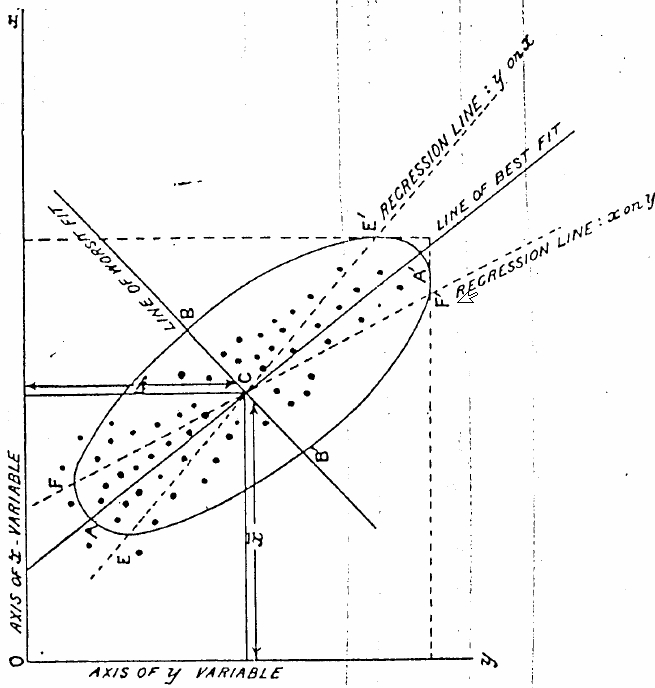
\includegraphics[width=10cm, height=9cm]{pearson}\\
    Wikimedia Commons: Karl Pearson, line of best fit diagram from Philosophical Magazine, 1901.
\end{center}
L'analyse en composantes principales a ses utilités hors du contexte du machine learning, en traitement du signal par exemple où \textit{la méthode des moindres carrés} permet de décomposer toute fonction périodique en une somme de $\cos$ et de $\sin$ plus faciles à traiter. Ceci permettra par exemple \textit{d'échantilloner} un signal continu tel qu'un son pour lui appliquer des traitements avant de le reconstituer. Dès votre premier semestre, en cours d'algèbre linéaire, il est possible que vous traitiez de la \textit{régression linéaire} comme application directe de la méthode des moindres carrés qui y sera présentée.\\

\noindent Ici, bien entendu, nous n'avons même pas égratigné l'iceberg des applications de l'algèbre linéaire, nous pourrions y passer des heures.

\subsection{Qu'est-ce que l'algèbre linéaire ?}
C'est, pragmatiquement, une branche des mathématiques très bien comprise, dans le sens : mieux comprise que nombre d'autres qui réservent davantage de mystères et hypothèses pas encore prouvées. On y étudie comment généraliser l'intuition géométrique acquise dans la géométrie planaire et la géométrie dans l'espace, et ce que cette généralisation apporte.\\

\noindent Ce cours introductif, comme le cours d'Algèbre Linéaire de l'EPFL, fera les hypothèses les plus minimes possibles sur vos apprentissages précédents de la matière. Ainsi, nous ne supposerons \textit{pas} que vous savez ce qu'est une matrice, encore moins un espace vectoriel, et nous repartons de zéro dès la section suivante.\\

\section{Prérequis sur les ensembles, fonctions et matrices}

Les trois premiers points de cette sous-section ne concernent pas spécifiquement l'algèbre linéaire mais vous serviront dans tout cours de maths. Le cours d'algèbre linéaire étant le premier de la prérentrée, nous avons jugé utile de placer ces sections ici plutôt que plus tard, d'autant plus qu'il faut les maîtriser pour continuer sur des bases solides en algèbre linéaire. Ainsi, vous savez peut-être déjà une grande partie de ce qui suit mais sûrement pas absolument tout.

\subsection{Opérations élémentaires sur les ensembles, dont le produit cartésien}
Dans ce cours comme tous les cours EPFL hormis ceux traitant justement de théorie des ensembles, nous dirons simplement et naïvement qu'\textbf{un ensemble est une collection d'éléments uniques et non ordonnés}. Dans la suite, nous notons, $A$ étant un ensemble, que $a \in A \iff$ (si et seulement si) l'élément $a$ appartient à l'ensemble $A$.\\

\noindent Pour caractériser un ensemble, il suffit par exemple:
\begin{itemize}
    \item de lister tous ses éléments : $\{1, 2\}$, $\{\text{chaussette rouge, chaussette verte}\}$, ...
    \item de le définir comme \textit{sous-ensemble} d'un ensemble connu en ajoutant une propriété, parfois appelée propriété bâtisseuse notée après une barre verticale : $\{ n \in \mathbb{N} \ | \ n \text{ divise 5}\}$ est l'ensemble des diviseurs naturels de 5, où $\mathbb{N} = \{0, 1, 2, ...\}$. Nous dirons au passage qu'un ensemble $E$ est sous-ensemble d'un ensemble $F$ si $E \subseteq F$, i.e si $E$ est inclus dans $F$, plus explicitement :
    $$E \subseteq F \iff \forall \text{ (pour tout) } e \in E, \ e \in F$$
    
    \item de le construire par union, intersection, complément, différence, produit cartésien entre ensembles.
\end{itemize}
Détaillons le dernier point. Soient deux ensembles $A$ et $B$, sous-ensembles de $X$. Alors nous pouvons définir :
\begin{itemize}
    \item \textit{L'union} de $A$ et $B$, notée $A \cup B = \{x \in X \ | \ x \in A \text{ ou }x \in B\}$.
    \item \textit{L'intersection} de $A$ et $B$, notée $A \cap B = \{x \in X \ | \ x \in A \text{ et } x \in B\}$.
    \item \textit{Le complément} de $A$, notée $\Bar{A} = \{x \in X \ | \ x \notin A\}$. Remarquons que $A \cup \Bar{A} = X$ et $A \cap \Bar{A} = \emptyset$, l'ensemble vide.
    \item \textit{La différence} de $A$ et $B$, notée $A \setminus B = A \cap \Bar{B}$.
    \item \textit{Le produit cartésien} de $A$ et $B$, qui nous intéressera particulièrement dans la suite, est noté $A \times B = \{(a,b) \ | \ a \in A, b \in B\}$ où $(a,b)$ est une \text{paire ordonnée} - en particulier $(a,b) \neq (b,a)$. Formellement, nous pourrions définir que $(a,b) = \{\{a\}, \{a,b\}\}$.\\
    \textit{Attention, $A$ n'est \textbf{pas} un sous-ensemble de $A \times B$}, $A \times B$ est constitué de paires, et pas $A$.\\
    Pour des ensembles $A_1, A_2,..., A_n$, nous pouvons définir leur produit cartésien ainsi, avec $\Iintv{1, n} = \{i \in \mathbb{N} \ | \ 1 \leq i \text{ et } i \leq n\}$ pour $n \in \mathbb{N}$ : $$A_1 \times A_2 \times ... \times A_n = \{(a_1, a_2, ..., a_n) \ | \ \forall i \in \Iintv{1, n}\ a_i \in A_i\}$$
\end{itemize}


\subsection{Définition d'une application ensembliste, ou fonction}
Dans cette section, notre seul objectif sera de définir formellement ce qu'est une \textit{application ensembliste}, autrement dit \textit{une fonction}. \\
La notion préliminaire est celle de \textit{relation} entre deux ensembles $A$ et $B$ : nous nommerons tout sous-ensemble $F$ de $A \times B$ une relation entre $A$ et $B$. Ensuite, nous dirons, concernant cette relation $F$, que :
$$F \text{ est une fonction de }A\text{ vers }B \iff \forall a \in A\ \exists! \text{ (il existe un unique) } b := F(a) \in B \text{ tel que } (a, F(a)) \in F
$$
Nous notons alors :
\begin{align*}
    F: \ &A \to B\\
    &a \mapsto F(a)
\end{align*}
En d'autres termes, pour chaque $a \in A$, un unique $F(a) \in B$ lui est associé, ce qui devrait correspondre à la définition de fonction donnée au gymnase, au lycée, ...

\subsection{Injectivité, surjectivité, bijectivité}
\noindent Cette section devrait contenir du contenu nouveau pour beaucoup.\\

\noindent Soit $f: A \to B$ une fonction. Nous définissons son \textit{injectivité} :
\begin{center}
    $f$ est \textit{injective} $\iff \forall a_1 \in A \ \forall a_2 \in A \ a_1 \neq a_2 \implies f(a_1) \neq f(a_2)$.\\
    
    De manière équivalente, en usant de la contraposée :\\
    
    $f$ est \textit{injective} $\iff \forall a_1 \in A \ \forall a_2 \in A \ f(a_1) = f(a_2) \implies a_1 = a_2$.
\end{center}
Ceci signifie que pour chaque $b \in B$, il existe \textit{au plus un} $a \in A$ tel que $f(a) = b$. Ainsi, si $A = \{a_1, a_2, a_3\}$ et $B = \{b_1, b_2, b_3, b_4\}$, voici une relation sur $A$ et $B$ définissant une fonction injective :

\begin{center}
\begin{tikzpicture}
  [scale=.6,auto=right]
      \node[vertex] (a1) at (1,10)  {$a_1$};
      \node[vertex] (a2) at (1,8)  {$a_2$};
      \node[vertex] (a3) at (1,6)  {$a_3$};
      \node[vertex] (b1) at (8,10)  {$b_1$};
      \node[vertex] (b2) at (8,8)  {$b_2$};
      \node[vertex] (b3) at (8,6)  {$b_3$};
      \node[vertex] (b4) at (8,4)   {$b_4$};

     \draw[->] (a1)--(b2);
     \draw[->] (a2)--(b3);
     \draw[->] (a3)--(b4);
\end{tikzpicture}
\end{center}

\noindent En effet, à chaque $b_i$ est associé au plus un $a_i$, le fait que $b_1$ n'ait pas d'antécédent ne nuit pas à l'injectivité. Cependant, la relation suivante sur $A$ et $B$ définit bien une fonction, mais pas une fonction injective :

\begin{center}
\begin{tikzpicture}
  [scale=.6,auto=right]
      \node[vertex] (a1) at (1,10)  {$a_1$};
      \node[vertex] (a2) at (1,8)  {$a_2$};
      \node[vertex] (a3) at (1,6)  {$a_3$};
      \node[vertex] (b1) at (8,10)  {$b_1$};
      \node[vertex] (b2) at (8,8)  {$b_2$};
      \node[vertex] (b3) at (8,6)  {$b_3$};
      \node[vertex] (b4) at (8,4)   {$b_4$};

     \draw[->] (a1)--(b2);
     \draw[->] (a2)--(b2);
     \draw[->] (a3)--(b4);
\end{tikzpicture}
\end{center}
Cette relation définit une fonction non injective car il existe 2 $a_i$, $a_1$ et $a_2$, qui ont pour image $b_2$.\\

\noindent Sur des exemples plus réalistes témoignant l'importance des ensembles de départ et d'arrivée :\\
$f: \R \to \R, x \mapsto x^2$ n'est pas injective, car tout réel positif non nul admet 2 antécédents par $f$: $x = f(\sqrt{x}) = f(-\sqrt{x})$. Au passage, $\R$ est l'ensemble des nombres réels.
\begin{center}
\begin{tikzpicture}
    \begin{axis}[
        xmin=-2,xmax=2,
        ymin=-2,ymax=2,
        axis x line=middle,
        axis y line=middle,
        axis line style=->,
        xlabel={$x$},
        ylabel={$y$},
        ]
\addplot[no marks,black,-] expression[domain=-2:2,samples=100]{x^2};
    \end{axis}
\end{tikzpicture}
\end{center}

\noindent Cependant, $g: \R^+ \to \R, x \mapsto x^2$ est bien injective, car nous avons limité le domaine de départ (aussi appelé domaine de définition) afin de faire en sorte qu'au plus un antécédent existe pour toute image.

\begin{center}
\begin{tikzpicture}
    \begin{axis}[
        xmin=0,xmax=2,
        ymin=-2,ymax=2,
        axis x line=middle,
        axis y line=middle,
        axis line style=->,
        xlabel={$x$},
        ylabel={$y$},
        ]
\addplot[no marks,black,-] expression[domain=0:2,samples=100]{x^2};
    \end{axis}
\end{tikzpicture}
\end{center}

\noindent Passons à la seconde définition importante concernant les fonctions, celle de \textit{surjectivité}.\\
Soit $f: A \to B$ une fonction :
$$f \text{ est \textit{surjective} } \iff \forall b \in B \ \exists \text{ (existe au moins un) }a \in A \text{ tel que } f(a) = b
$$
Ceci signifie... rien de plus que la définition : pour chaque $b \in B$, il existe \textit{au moins} un $a \in A$ tel que $f(a) = b$. Le "au moins" est important, ainsi la fonction suivante est surjective avec $A = \{a_1, ..., a_4\}$ et $B = \{b_1, b_2, b_3\}$ :

\begin{center}
\begin{tikzpicture}
  [scale=.6,auto=right]
      \node[vertex] (a1) at (1,10)  {$a_1$};
      \node[vertex] (a2) at (1,8)  {$a_2$};
      \node[vertex] (a3) at (1,6)  {$a_3$};
      \node[vertex] (a4) at (1,4)  {$a_4$};
      \node[vertex] (b1) at (8,10)  {$b_1$};
      \node[vertex] (b2) at (8,8)  {$b_2$};
      \node[vertex] (b3) at (8,6)  {$b_3$};

     \draw[->] (a1)--(b1);
     \draw[->] (a2)--(b2);
     \draw[->] (a3)--(b3);
     \draw[->] (a4)--(b3);
\end{tikzpicture}
\end{center}
Elle est surjective car au moins un $a_i$ pointe vers chaque $b_j$. Notons qu'elle n'est pas injective car $a_3$ et $a_4$ ont l'image commune $b_3$. Si nous rajoutions un $b_4$ sans lui lier de $a_i$, la fonction obtenue ne serait plus surjective, ce $b_4$ n'admettant pas d'antécédent.\\

\noindent Avant d'arriver à des exemples plus réalistes, définissons \textit{l'ensemble image} d'une fonction $f: A \to B$. Etant donné un sous-ensemble $S \subseteq A$, nous définissons : 
$$f(S) = \{b \in B \ | \ \exists s  \in S  \ f(s) = b\}
$$
L'image de $f$ sera alors :
$$\Ima(f) = f(A) = \{ b \in B \ | \ \exists a \in A \ f(a) = b \}
$$
Ainsi, étant donnée une telle fonction $f$, nous pouvons restreindre son domaine d'arrivée afin de la rendre surjective : $g: A \to \Ima(f), x \mapsto f(x)$ est surjective par définition.\\

\noindent En fait, nous pouvons même définir la surjectivité autrement mais de manière équivalente grâce à cet ensemble image :
$$f: A \to B \text{ est surjective } \iff \Ima(f) = B
$$

\noindent Pour retourner à l'exemple de fonctions associant des carrés à des antécédents : soit $f : \R \to \R^+, x \mapsto x^2$, cette fonction est surjective puisque pour tout $x \geq 0 \ \exists y \in \R$ tel que $f(y) = x$, et ce $y = \sqrt{x}$ :
\begin{center}
\begin{tikzpicture}
    \begin{axis}[
        xmin=-2,xmax=2,
        ymin=0,ymax=2,
        axis x line=middle,
        axis y line=middle,
        axis line style=->,
        xlabel={$x$},
        ylabel={$y$},
        ]
\addplot[no marks,black,-] expression[domain=-2:2,samples=100]{x^2};
    \end{axis}
\end{tikzpicture}
\end{center}
La même fonction à laquelle on associerait le domaine d'arrivée $\R$ voire même $\C$ sans changer le domaine de définition deviendrait non surjective, car pour $b = -1$ par exemple, il n'existe pas de $a$ réel tel que $a^2 = -1$.\\

\noindent Dernière définition de cette section, la \textit{bijectivité}. Soit $f: A \to B$ une fonction :
\begin{align*}
    f \text{ est bijective } &\iff f \text{ est injective et surjective}\\
    &\iff \forall b \in B\ \exists! a \in A \ f(a) = b
\end{align*}
Pour reprendre une dernière fois nos petites fonctions avec des flèches, avec cette fois $A = \{a_1, a_2, a_3\}$ et $B = \{b_1, b_2, b_3\}$, la fonction suivante est bijective :

\begin{center}
\begin{tikzpicture}
  [scale=.6,auto=right]
      \node[vertex] (a1) at (1,10)  {$a_1$};
      \node[vertex] (a2) at (1,8)  {$a_2$};
      \node[vertex] (a3) at (1,6)  {$a_3$};
      \node[vertex] (b1) at (8,10)  {$b_1$};
      \node[vertex] (b2) at (8,8)  {$b_2$};
      \node[vertex] (b3) at (8,6)  {$b_3$};

     \draw[->] (a1)--(b2);
     \draw[->] (a2)--(b1);
     \draw[->] (a3)--(b3);
\end{tikzpicture}
\end{center}
Elle vérifie bien injectivité et surjectivité. \\
Aussi, pour clore sur les fonctions associant des carrés, la fonction suivante est bijective, où nous avons réduit le domaine de départ pour la rendre injective, puis restreint le domaine d'arrivée pour la rendre surjective :\\
\begin{align*}
    f: \ &\R^+ \to \R^+ \\
    &x \mapsto x^2
\end{align*}
\begin{center}
\begin{tikzpicture}
    \begin{axis}[
        xmin=0,xmax=2,
        ymin=0,ymax=2,
        axis x line=middle,
        axis y line=middle,
        axis line style=->,
        xlabel={$x$},
        ylabel={$y$},
        ]
\addplot[no marks,black,-] expression[domain=0:2,samples=100]{x^2};
    \end{axis}
\end{tikzpicture}
\end{center}

\subsection{Définitions de $\R^n$, de matrice et du produit matrice-vecteur}
\noindent En algèbre linéaire, la fonction qui nous occupera longtemps - en fait tout le reste de ce cours préparatif - est la suivante, où $n,p \in \mathbb{N}_{\geq 1}$ :
\begin{align*}
    f: \ &\R^n \to \R^p\\
    &x \mapsto f(x) = Ax \text{ où $A$ est une matrice } p \times n
\end{align*}
Décortiquons cette fonction pas-à-pas.\\
D'abord, nous savons en fait ce qu'est $\R^n$ à présent : 
$$\R^n = \underbrace{\R \times \R \times ... \times \R}_{n \text{ fois}} = \{x=(x_1, x_2, ..., x_n) \ | \ \forall i \in \Iintv{1, n}\ x_i \in \R\}$$
Ainsi, $\R^2 = \R \times \R$ est, géométriquement, l'ensemble des points $(x,y)$ du plan, au même titre que $\R^3$ est l'ensemble des points $(x,y,z)$ de l'espace.\\
Nous nommerons l'ensemble des éléments de $\R^n$ des \textit{vecteurs}, ainsi $f$ associe des vecteurs de dimension $n$ à des vecteurs de dimension $p$, ok, désormais la question est comment... ?\\
Notons les vecteurs en colonnes ainsi: $x = (a,b,c) = \begin{bmatrix}a \\ b \\ c \end{bmatrix}$. Puis, soit $f: \R^3 \to \R^2$.\\
Considérons $f(x) = f\left(\begin{bmatrix}a \\ b \\ c \end{bmatrix} \right) = \begin{bmatrix}a+5b \\ 3a-b+2c \end{bmatrix}$. Mettons en évidence les coefficients devant $a, b$ et $c$ :
$$\begin{bmatrix}a+5b \\ 3a-b+2c \end{bmatrix} = \begin{bmatrix}1 \cdot a+5\cdot b + 0 \cdot c \\ 3 \cdot a + (-1) \cdot b+2 \cdot c \end{bmatrix} = \underbrace{\begin{bmatrix} 1 & 5 & 0 \\3 & -1 & 2 \end{bmatrix}}_{A_{2 \times 3}} \begin{bmatrix}a \\ b \\ c \end{bmatrix}
$$
Que signifie cette dernière égalité ? Ici, $A$ est une matrice $2 \times 3$, une matrice n'étant rien de plus qu'un tableau (fini) de nombres, ici, réels, de $p$ lignes (ici 2) et $n$ colonnes (ici 3). La dernière égalité use du \textit{produit matrice-vecteur} : En multipliant une matrice de taille $p \times n$ par un vecteur de dimension $n$, nous obtenons un vecteur de dimension $p$ tel que chaque $i$ème \textit{coordonnée} est le \textit{produit scalaire} de la $i$ème ligne de la matrice avec le vecteur. Ainsi :
$$Ax = \begin{bmatrix} a_{1,1} & a_{1,2} & \cdots & a_{1, n} \\ a_{2,1} & a_{2,2} & \cdots & a_{2, n} \\ \vdots & \ddots & & \vdots \\ a_{p,1} & \cdots & \cdots & a_{p,n} \end{bmatrix}\begin{bmatrix} x_1 \\ x_2 \\ \vdots \\ x_n \end{bmatrix} = \begin{bmatrix} a_{1,1}x_1 + a_{1,2}x_2 + a_{1,3}x_3 + ... + a_{1, n}x_n \\ a_{2,1}x_1 + a_{2,2}x_2 + a_{2,3}x_3 + ... + a_{2, n}x_n \\ \vdots \\ a_{p,1}x_1 + a_{p,2}x_2 + a_{p,3}x_3 + ... + a_{p, n}x_n \end{bmatrix} = \left[\sum_{k = 1}^n a_{i,k}x_k\right]_{i \in \Iintv{1,p}}
$$
Notons tout de suite que dans la fonction proposée $f: \R^n \to \R^p, x \mapsto Ax$, $n$ est le nombre de \textit{colonnes} de $A$ et $p$ son nombre de \textit{lignes}. En effet, une matrice prend des vecteurs de dimension son nombre de colonnes pour les associer à des vecteurs de dimension son nombre de lignes, donc l'application $f$ associée que nous nommerons \textit{application matricielle} ou fonction matricielle dans la suite a pour domaine de définition les vecteurs de dimension le nombre de colonnes, et pour domaine d'arrivée les vecteurs de dimension le nombre de lignes.\\

\noindent Remarquons qu'une matrice \textit{n'est pas} une simple notation, mais est bien un objet mathématique en tant que tel, qui pourrait être précisé ainsi : si $b_1, ..., b_n$ sont les colonnes d'une matrice $B$ de taille $p \times n$ - donc des vecteurs de dimension $p$, nous pourrions poser que $B = (b_1, ..., b_n)$ ainsi $B \in (\R^p)^n$ vu que $B$ est un $n$-tuple d'éléments d'un certain ensemble $E$, et $E$ se trouve être $\R^p$. Ceci donne une définition plus rigoureuse que celle d'un tableau de $pn$ entrées, mais nous privilégions néanmoins la notation du tableau car elle est plus intuitive. \\
Pour cette raison, nous notons l'ensemble des matrices de taille $p \times n$ à coefficients réels ainsi : $\R^{p \times n}$.\\
 
\newpage

\section*{Deuxième période, 9h15 à 10h}

\section{Systèmes linéaires}
\noindent Voyons ici une première application importante des objets mathématiques introduits dans la section précédente, les matrices : les \textit{systèmes d'équations linéaires}. Tout d'abord qu'est ce qu'une équation linéaire ? Il s'agit d'une égalité faisant intervenir une somme d'inconnues chacune multipliées par un coefficient réel. 

\subsection{Définition et exemples, intuition géométrique}
\noindent Plus formellement une équation linéaire est une équation de la forme : 
$$a_1 x_1 + ... + a_n x_n = b$$
avec $\{a_i \}_{i \in \Iintv{1,n}} \subseteq \mathbb{R}$ et $b\in \mathbb{R}$. Nous appelons $n$ le nombre \textit{d'inconnues}. Un \textit{système} d'équations linéaires est caractérisé par un ensemble \textit{fini} d'équations linéaires. Plus précisément nous pouvons donc représenter une équation linéaire sous la forme :
$$a_1 x_1 + ... + a_n x_n = b
$$
où les $a_i \in \R$ et $b \in \R$ sont connus, puis écrire un système linéaire :
$$\begin{cases} a_{1,1}x_1 + a_{1,2}x_2 + a_{1,3}x_3 + ... + a_{1, n}x_n = b_1 \\ a_{2,1}x_1 + a_{2,2}x_2 + a_{2,3}x_3 + ... + a_{2, n}x_n =b_2 \\ \vdots \\ a_{p,1}x_1 + a_{p,2}x_2 + a_{p,3}x_3 + ... + a_{p, n}x_n = b_p \end{cases}$$

\noindent Le plus souvent, la donnée intéressante d'un système d'équations linéaires est son ensemble de solutions, c'est à dire le tuple des $(y_1, y_2, \ldots, y_n)\in \mathbb{R}^n$ tels que pour chaque équation du système, en injectant ces valeurs dans les $x_n$ on obtienne bien $b_i$. Notons pour l'instant cet ensemble de solutions $S(\{a_{i,j}\},b)$. Concentrons-nous sur quelques équations simples pour visualiser géométriquement à quoi ressemblent ces ensembles de solutions.\\

\noindent Tout d'abord remarquons que pour un système d'équations à $n$ variables, $S(\{a_{i,j}\}, b)$ est un sous ensemble de $\mathbb{R}^n$ puisqu'il est constitué de $n$-uplets de réels. Commençons donc avec des sous ensembles de $\mathbb{R}^2$, à savoir des sous ensembles du plan. 
$$ 2x_1 - x_2 = 0 $$
\noindent Ceci est l'équation d'une droite. Ici nous commençons par remarquer qu'il s'agit d'un système à une équation et deux variables, nous avons, selon la notation précédente $a_{1,1} =2 $, $a_{1,2} = -1$ et  $b_1 = 0$. Lorsque tous les $b_i$ sont nuls nous dirons que le système d'équations est \textit{homogène}. Nous résolvons en passant simplement le $x_2$ de l'autre coté on obtient :
$$2x_1 = x_2$$
Il s'agit donc de l'ensemble des $(x_1, x_2) \in \mathbb{R}^2$ tels que $2x_1 = x_2$. Nous pourrons alors aussi dire qu'il s'agit, pour tout $x\in \mathbb{R}$ des $(x, 2x)$. Géométriquement à quoi correspond cet ensemble ? Remarquons que comme $x$ est réel il s'agit bien de l'ensemble des $\left\{x\begin{bmatrix}1 \\ 2 \end{bmatrix} \ | \ x \in \R\right\}$. Visuellement le vecteur $\begin{bmatrix}1 \\ 2 \end{bmatrix}$ est représenté ci dessous. L'ensemble des vecteurs obtenus en lui multipliant un réel $x$ sont représentés sur la figure de droite.
\begin{center}
\begin{tikzpicture}

  \draw[thin,gray!40] (-3,-3) grid (3,3);
  \draw[<->] (-3,0)--(3,0) node[right]{$x$};
  \draw[<->] (0,-3)--(0,3) node[above]{$y$};
  \draw[line width=2pt,blue,-stealth](0,0)--(1,2) node[anchor=south west]{$\begin{bmatrix}1 \\ 2 \end{bmatrix}$};
\end{tikzpicture}
\hspace{2CM}
\begin{tikzpicture}
  \draw[thin,gray!40] (-3,-3) grid (3,3);
  \draw[<->] (-3,0)--(3,0) node[right]{$x$};
  \draw[<->] (0,-3)--(0,3) node[above]{$y$};
    \draw[line width=2pt,red,-stealth](0,0)--(1.5,3) node[anchor=south west]{};
  \draw[line width=2pt,blue,-stealth](0,0)--(1,2) node[anchor=south west]{};
  \draw[line width=2pt,red,-stealth](0,0)--(-1.5,-3) node[anchor=south west]{};

\end{tikzpicture}
\end{center}
Il s'agit donc d'une droite dirigée par le vecteur $\begin{bmatrix}1 \\ 2 \end{bmatrix}$. Prenons désormais un exemple avec un système à trois inconnues et deux équations :

$$ \begin{cases}3x_1 + 2x_2 + x_3 = 2\\x_1 + 2x_2 + x_3 = 2 \end{cases}$$
%yeet
%who is the author of this yeet?
Comment procéder à la résolution ? Soustrayons la deuxième équation à la première pour obtenir :

$$ \begin{cases}2x_1  = 0\\ x_1 + 2x_2 + x_3 = 2 \end{cases}$$

\noindent Et donc conclure déjà que les points de notre ensemble de solution seront de la forme $(0, x_2, x_3)\in \mathbb{R}^3$ en divisant des deux cotés de $ 2x_1  = 0$ par $2$. Remplaçons donc $x_1$ par $0$ dans la seconde équation pour obtenir :
$$ 2x_2 + x_3 = 2 $$
\noindent Il s'agit encore une fois de l'équation d'une droite, ici de la droite dirigée par $$\begin{bmatrix}0 \\ 1 \\ -2 \end{bmatrix}$$ mais décalée de $2$ au niveau de l'origine :
\\
\begin{tikzpicture}

\pgfplotsset{
colormap={whitered}{color(0cm)=(white); color(1cm)=(orange!75!red)}
}

\begin{axis}[  colormap name=whitered,   view={45}{65},     width=10cm]
\addplot3[variable=t, mesh, draw=red!50, domain=-2:2] (0,{t + 2},{-2*t});
\end{axis}
\end{tikzpicture}
\hspace{1CM}
\begin{tikzpicture}
  \draw[thin,gray!40] (-3,-3) grid (3,3);
  \draw[<->] (-3,0)--(3,0) node[right]{$x$};
  \draw[<->] (0,-3)--(0,3) node[above]{$y$};
    \draw[line width=2pt,red,-stealth](-0.25,3)--(2.25,-3) node[anchor=south west]{};

\end{tikzpicture}
A droite est une coupe selon l'axe des $x_1 = 0$. 
\subsection{L'équation $Ax = b$}
\noindent Reprenons une équation connue et cherchons les informations capitales à son sujet : 
$$ \begin{cases}5x_1 + x_3 = \sqrt{2}\\x_1 + 3x_2 +4x_3 = 3\end{cases} $$
\noindent Quelles sont les informations minimales dont on a besoin pour reconstituer une telle équation ? Les variables peuvent être ordonnées de sorte à toujours apparaître dans le même ordre. Nous pourrions aussi omettre le signe "$=$" en sachant que le dernier coefficient est celui correspondant à $b_i$. Enfin nous pourrions encore omettre le nom des variables et ne conserver que les coefficients puisque l'ordre des coefficients détermine la variable qu'ils multiplient. Et que faire si l'une des variables n'est pas présente ? Il s'agit bien de la multiplication par $0$ dans ce cas. En résumé nous obtenons :
$$ 5 \quad 0 \quad 1 \quad \sqrt{2}$$
$$ 1 \quad 3 \quad 4 \quad 3 $$
Nous pouvons réécrire cela de manière plus élégante sous la forme :
$$ 
\left[
\begin{array}{@{}ccc|c@{}}
5 & 0 & 1 & \sqrt{2} \\
1 & 3 & 4 & 3 \\
\end{array}
\right]
$$
\noindent Voici la forme \textit{matricielle augmentée} d'un système linéaire. Cette forme est équivalente à la donnée de l'équation suivante dite \textit{équation matricielle} $Ax = b$ :
$$\underbrace{\begin{bmatrix}
5 & 0 & 1 \\
1 & 3 & 4 
\end{bmatrix}}_{A}\underbrace{\begin{bmatrix}
x_1 \\ x_2 \\ x_3
\end{bmatrix}}_{x} = \underbrace{\begin{bmatrix}
\sqrt{2} \\ 2
\end{bmatrix}}_{b}
$$
Dans cette notation, $A$ est la \textit{matrice des coefficients}, et la \textit{matrice augmentée} de l'équation matricielle est ainsi $\begin{bmatrix}
A & | & b
\end{bmatrix}$.

\subsection{Réduction et échelonnage}
\noindent Soit le système linéaire :
$$\begin{cases}
3x_1 + 2x_2 + x_3 = 2\\
x_1 + 2x_2 + x_3 = 2
\end{cases}
$$
La matrice augmentée associée est alors :
$$ 
\left[
\begin{array}{@{}ccc|c@{}}
3 & 2 & 1 & 2 \\
1 & 2 & 1 & 2 \\
\end{array}
\right]
$$
Résolvons ce système sous les deux écritures i.e système et matrice augmentée simultanément. Soustrayons donc chaque coefficient de la seconde ligne au coefficient correspondant de la ligne supérieure pour obtenir :
$$ 
\left[
\begin{array}{@{}ccc|c@{}}
3 \color{red} - 1 & 2 \color{red} -2 & 1  \color{red} - 1 & 2 \color{red} - 2 \\
1 & 2 & 1 & 2 \\
\end{array}
\right] 
\iff 
\begin{cases}
(3\textcolor{red}{-1})x_1 + (2\textcolor{red}{-2})x_2 + (1\textcolor{red}{-1})x_3 = 2\textcolor{red}{-2}\\
x_1 + 2x_2 + x_3 = 2
\end{cases}
$$

$$ 
\left[
\begin{array}{@{}ccc|c@{}}
2 & 0 & 0 & 0 \\
1 & 2 & 1 & 2 \\
\end{array}
\right]
\iff
\begin{cases}
2x_1 = 0\\
x_1 + 2x_2 + x_3 = 2
\end{cases}
$$
Nous multiplions ensuite les coefficients de la première ligne par $\color{blue}\frac{1}{2}$ :
$$ 
\left[
\begin{array}{@{}ccc|c@{}}
2 \color{blue}\times\frac{1}{2}  & 0 & 0 & 0 \\
1 & 2 & 1 & 2 \\
\end{array}
\right]
\iff
\begin{cases}
2\textcolor{blue}{\times \frac{1}{2}}x_1 = 0\\
x_1 + 2x_2 + x_3 = 2
\end{cases}
$$
$$ 
\left[
\begin{array}{@{}ccc|c@{}}
1 & 0 & 0 & 0 \\
1 & 2 & 1 & 2 \\
\end{array}
\right]
\iff
\begin{cases}
x_1 = 0 \\
x_1 + 2x_2 + x_3 = 2
\end{cases}
$$
Et nous concluons alors que le premier coefficient est nul.\\
Continuons en soustrayant la première ligne à la seconde :
$$ 
\left[
\begin{array}{@{}ccc|c@{}}
1 & 0 & 0 & 0 \\
1\color{red} - 1 & 2\color{red} - 0 & 1\color{red} - 0 & 2\color{red} - 0 \\
\end{array}
\right]
\iff 
\begin{cases}
x_1 = 0 \\
(1\textcolor{red}{-1})x_1 + (2\textcolor{red}{-0})x_2 + (1\textcolor{red}{-0})x_3 = 2\textcolor{red}{-0}
\end{cases}
$$
$$ 
\left[
\begin{array}{@{}ccc|c@{}}
1 & 0 & 0 & 0 \\
0 & 2 & 1 & 2 \\
\end{array}
\right]
\iff
\begin{cases}
x_1 = 0 \\
2x_2 + x_3 = 2
\end{cases}
$$
Nous pouvons peut être aller un peu plus loin en divisant la deuxième ligne par 2, ce qui donne :
$$
\left[
\begin{array}{@{}ccc|c@{}}
1 & 0 & 0 & 0 \\
0 & 1 & \frac{1}{2} & 1 \\
\end{array}
\right]
\iff
\begin{cases}
x_1 = 0 \\
x_2 + \frac{1}{2}x_3 = 1
\end{cases}
$$
Formalisons les opérations que nous pouvons utiliser pour résoudre un système linéaire sous sa forme matricielle, qui sont en fait les mêmes que celle sous sa forme de système d'équations linéaires : 
\begin{itemize}
    \item \textit{La multiplication par un réel non nul} d'une ligne complète (ne pas oublier le $b_i$).
    \item \textit{Additionner deux lignes} puisque la soustraction correspond à multiplier la ligne par $-1$ puis l'additionner à l'autre et la multiplier à nouveau par $-1$.
    \item \textit{Permuter deux lignes}, la permutation de deux équations dans un système étant sans conséquence.
\end{itemize}
\textbf{Notons d'abord que ces trois opérations sont réversibles. C'est ce qui fait que l'ensemble des solutions n'est pas changé par ces 3 opérations.}\\

\noindent Remarquons aussi que nous pouvons toujours procéder comme dans la soustraction et multiplier la $i$ème ligne par un réel $\lambda \in \mathbb{R}^*$, l'additionner à la $j$-ème ligne et multiplier à nouveau la $i$ème ligne par $\frac{1}{\lambda}$. Nous en concluons une règle composite très pratique : 
\begin{itemize}
    \item \textit{La multiplication puis l'addition} d'une ligne vers une autre sans modifier sa propre valeur.
\end{itemize}
Il s'agit désormais de trouver un algorithme qui pourrait toujours mener vers la forme la plus réduite possible d'une équation, commençons par trouver les critères qu'une telle forme doit posséder. Tout d'abord on remarque que les lignes de la forme 
$$ 
\left[
\begin{array}{@{}ccccc|c@{}}
0 & \ldots & \lambda & \ldots & 0 & \sigma \\
\end{array}
\right]
\iff
0x_1 + \cdots + \lambda x_i + 0x_{i+1} + \cdots + 0x_n = \sigma
$$
pour tout $\lambda \in \R^*, \sigma \in \mathbb{R}$ sont très pratiques puisqu'elles déterminent la valeur de la variable dont le coefficient n'est pas nul de manière unique : $x_i = \frac{\sigma}{\lambda}$. Il s'agirait donc d'obtenir une matrice qui maximise le nombre de ligne de cette forme.\\

\noindent Remarquons que si nous disposons d'une ligne de la forme :
$$ 
\left[
\begin{array}{@{}ccccc|c@{}}
0 & \ldots & \lambda_1 & \ldots & \lambda_n & \sigma \\
\end{array}
\right]
$$
\noindent Alors pour annuler les derniers coefficients (sur la droite) il faut déjà avoir une ligne qui contienne au plus autant de coefficients non nuls à droite sans quoi lors de l'addition des lignes nous créerons des termes non nuls là où nous avions déjà des termes nuls :
$$ 
\left[
\begin{array}{@{}ccccc|c@{}}
0 \color{green} -0  & 0\color{green} -0 & \lambda_1 \color{green} -\alpha_1 & \lambda_2 \color{green} -\alpha_2 & \lambda_3\color{green} -\alpha_3 & \sigma_1\color{green} -\sigma_2 \\
0 & 0  & \alpha_1 & \alpha_2 & \alpha_3 & \sigma_2 \\
\end{array}
\right]
$$
Ci-dessus une soustraction n'ajoutant pas de termes, et ci après une soustraction ajoutant des termes non nuls.
$$ 
\left[
\begin{array}{@{}ccccc|c@{}}
0 \color{green} -0  & 0\color{red} -\alpha_0 & \lambda_1 \color{green} -\alpha_1 & \lambda_2 \color{green} -\alpha_2 & \lambda_3\color{green} -\alpha_3 & \sigma_1\color{green} -\sigma_2 \\
0 & \alpha_0  & \alpha_1 & \alpha_2 & \alpha_3 & \sigma_2 \\
\end{array}
\right]
$$
Nous constatons donc que pour arriver à obtenir une forme matricielle contenant le plus de lignes avec un seul terme non nul il conviendrai premièrement d'en trouver une dont les lignes auraient un \textit{nombre de termes non nul à droite décroissant}, c'est-à-dire telle que : si $A \in \R^{p \cross n}$, alors pour tout $i \in \Iintv{1,p}$, si la colonne $k\in \Iintv{1,n}$ est la première colonne de la $i$ème ligne dont le coefficient est non nul, alors le rang de la première colonne de la $i+1$ème ligne dont le coefficient est non nul est strictement supérieur à $k$. Dans la matrice suivante, $*$ désigne un coefficient arbitraire, et $\Delta$ un coefficient \textit{non nul} arbitraire.
$$\begin{bmatrix}
0 & \cdots & 0 & \Delta & * & \cdots & * & * & *\\
0 &\cdots & 0 & 0 & \cdots & \Delta & * &\cdots & *\\
\vdots &&&&&&&&\vdots \\
0 & &&\cdots&&\cdots&&& *
\end{bmatrix}
$$
Nous appelons cette forme la forme \textit{échelonnée} d'une matrice. Les premiers termes non nuls sur une ligne sont appelés \textit{pivots}. \\
En d'autres termes, les coefficients non nuls font une sorte d'escalier plus ou moins régulier. Des exemples de matrices sous forme échelonnée, avec, en bleu, les pivots :
$$
\begin{bmatrix}
\color{blue}5 & 0 & 3 & 3 \\
0 & 0 & \color{blue}2 & 1 \\
0 & 0 & 0 & 0
\end{bmatrix},
\begin{bmatrix}
0 & 0 \\
0 & 0
\end{bmatrix},
\begin{bmatrix}
\color{blue}1 & 0\\
0 & \color{blue}1\\
0 & 0
\end{bmatrix},
\begin{bmatrix}
0 & 0 & 0 & 0 & 0 \\
0 & 0 & 0 & \color{blue}5 & 4
\end{bmatrix}
$$
Des exemples de matrices \textit{pas} sous forme échelonnée :
$$
\begin{bmatrix}
0 & 2 & 3 \\
1 & 5 & 6\\
0 & 9 & 1
\end{bmatrix},
\begin{bmatrix}
0 & 0 & 7 \\
0 & 4 & 0\\
0 & 0 & 0\\
0 & 0 & 0
\end{bmatrix}
$$
La première n'est pas échelonnée car le coefficient $1$ est en colonne $1$ de la ligne 2, soit avant le premier coefficient non nul de la ligne au-dessus, qui est $2$. Idem : le $4$ dans la seconde matrice est situé à la deuxième colonne alors que la première ligne compte le coefficient non nul 7 à la troisième colonne.\\

\noindent Ensuite, étant donnée une forme échelonnée, il est encore possible de la réduire. Nous pouvons faire en sorte que tous les pivots valent $1$ et que tous les coefficients sur la même colonne au-dessus de chaque pivot deviennent nuls, et ce \textit{en divisant la ligne du pivot} par le pivot lui-même (non nul par définition), puis en soustrayant la ligne du pivot aux lignes du dessus. Ainsi, il faudra commencer par la ligne du-dessous.\\
Nous appelons cette forme celle de matrice \textit{échelonnée réduite}.\\
Des exemples rendront ce texte cryptique  plus compréhensible :
\begin{align*}
\begin{bmatrix}
\color{blue}5 & 0 & 3 & 3\\
0 & 0 & \color{blue}2 & 1\\
0 & 0 & 0 & 0
\end{bmatrix} \overset{L_2 \to  \frac{1}{2}L_2}{\sim} 
&\begin{bmatrix}
\color{blue}5 & 0 & 3 & 3\\
0 & 0 & \color{blue}1 & \frac{1}{2}\\
0 & 0 & 0 & 0
\end{bmatrix}\\
\overset{L_1 \to L_1 - 3L_2}{\sim}
&\begin{bmatrix}
\color{blue}5 & 0 & 0 & \frac{3}{2}\\
0 & 0 & \color{blue}1 & \frac{1}{2}\\
0 & 0 & 0 & 0
\end{bmatrix}\\
\overset{L_1 \to \frac{1}{5}L_1}{\sim}
&\begin{bmatrix}
\color{blue}1 & 0 & 0 & \frac{3}{10}\\
0 & 0 & \color{blue}1 & \frac{1}{2}\\
0 & 0 & 0 & 0
\end{bmatrix}
\end{align*}
Puis, $\begin{bmatrix}
0 &0\\
0 & 0
\end{bmatrix}$ est déja échelonnée réduite. Idem, la matrice $\begin{bmatrix}
1 & 0\\
0 & 1\\
0 & 0
\end{bmatrix}$ l'est déjà aussi. Enfin :
\begin{align*}
\begin{bmatrix}
0 & 0 & 0 & 0 & 0 \\
0 & 0 & 0 & \color{blue}5 & 4
\end{bmatrix}
\overset{L_2 \to \frac{1}{5}L_2}{\sim}
\begin{bmatrix}
0 & 0 & 0 & 0 & 0 \\
0 & 0 & 0 & \color{blue}1 & \frac{4}{5}
\end{bmatrix}
\end{align*}
Nous verrons dans la prochaine section comment exploiter cette forme échelonnée réduite afin d'expliciter l'ensemble des solutions d'un système linéaire.\\

\noindent Il serait désormais utile de trouver un algorithme amenant à une forme échelonnée, puisque nous savons passer d'une forme échelonnée à une forme réduite désormais. La méthode présentée ci-après est celle du \textit{pivot de Gauss}.\\

\noindent Nous commencerons par un exemple. Calculons la forme échelonnée réduite de la matrice suivante :
$$\begin{bmatrix}
-1 & -2 & -1 & 3 \\
-2 & -3 &  0 & 3 \\
1  &  4 &  5 & -9
\end{bmatrix}
$$
\begin{mdframed}
Le but sera d'aller de la gauche vers la droite. Pour chaque colonne, nous sélectionnerons une ligne que nous trouverions "avantageuse" afin de simplifier les calculs, bien qu'en soi n'importe quelle ligne marcherait. Cette ligne sera placée au-dessus. Puis, nous ajoutons des multiples de cette ligne aux lignes en-dessous de manière à faire apparaître des 0 dans la colonne courante. Puis, nous bloquons la ligne du dessus et passons à la prochaine colonne jusqu'à arriver avoir traité la colonne la plus à droite.
\end{mdframed}

\noindent Ici, en choisissant la 3ème ligne dans la matrice ci-dessus, i.e celle contenant un coefficient $1$ à sa gauche, nous pourrions simplement annuler le $-1$ et le $-2$ en ajoutant respectivement 1 et 2 fois la ligne 3. Au fur et à mesure, les pivots bloqués seront colorés en bleu.\\

\noindent Chaque chose en son temps. Mettons d'abord en évidence cette ligne 3 en la plaçant au-dessus :
$$\begin{bmatrix}
-1 & -2 & -1 & 3 \\
-2 & -3 &  0 & 3 \\
1  &  4 &  5 & -9
\end{bmatrix}
\overset{L_1 \leftrightarrow L_3}{\sim} 
\begin{bmatrix}
\color{blue}1  &  4 &  5 & -9\\
-2 & -3 &  0 & 3 \\
-1 & -2 & -1 & 3 
\end{bmatrix}
$$
Ensuite, faisons des $0$ apparaître sous ce premier futur pivot :
\begin{align*}
\begin{bmatrix}
\color{blue}1  &  4 &  5 & -9\\
-2 & -3 &  0 & 3 \\
-1 & -2 & -1 & 3 
\end{bmatrix}
\overset{L_2 \to L_2 + 2L_1}{\sim}
&\begin{bmatrix}
\color{blue}1  &  4 &  5 & -9\\
0 & 5 &  10 & -15 \\
-1 & -2 & -1 & 3 
\end{bmatrix}\\
\overset{L_3 \to L_3 + L_1}{\sim}
&\begin{bmatrix}
\color{blue}1  &  4 &  5 & -9\\
0 & 5 &  10 & -15 \\
0 & 2 & 4 & -6 
\end{bmatrix}
\end{align*}
Nous pourrions recommencer directement l'opération avec la seconde colonne comme le prescrit la méthode de Gauss, mais remarquons d'abord que les lignes 2 et 3 se ressemblent particulièrement et sont toutes deux multiples de $\begin{bmatrix}
0 & 1 & 2 & -3
\end{bmatrix}$, mettons cela en évidence :
\begin{align*}
\begin{bmatrix}
\color{blue}1  &  4 &  5 & -9\\
0 & 5 &  10 & -15 \\
0 & 2 & 4 & -6 
\end{bmatrix}
\overset{L_3 \to \frac{1}{2}L_3}{\sim}
&\begin{bmatrix}
\color{blue}1  &  4 &  5 & -9\\
0 & 5 &  10 & -15 \\
0 & 1 & 2 & -3 
\end{bmatrix}\\
\overset{L_2 \to \frac{1}{5}L_2}{\sim}
&\begin{bmatrix}
\color{blue}1  &  4 &  5 & -9\\
0 & 1 & 2 & -3 \\
0 & 1 & 2 & -3 
\end{bmatrix}
\end{align*}
Il ne reste plus qu'à \textbf{YEET} la 2ème ligne - c'est un terme technique signifiant soustraire la 3ème à la 2ème ;)
$$
\begin{bmatrix}
\color{blue}1  &  4 &  5 & -9\\
0 & 1 & 2 & -3 \\
0 & 1 & 2 & -3 
\end{bmatrix}
\overset{L_2 \to L_2 - L_3}{\sim}
\begin{bmatrix}
\color{blue}1  &  4 &  5 & -9\\
0 & 0 & 0 & 0 \\
0 & 1 & 2 & -3 
\end{bmatrix}
$$
Nous avons presque une forme échelonnée ! Il reste encore à permuter les deux dernières lignes :
$$
\begin{bmatrix}
\color{blue}1  &  4 &  5 & -9\\
0 & 0 & 0 & 0 \\
0 & 1 & 2 & -3 
\end{bmatrix}
\overset{L_2 \leftrightarrow L_3}{\sim}
\begin{bmatrix}
\color{blue}1  &  4 &  5 & -9\\
0 & \color{blue}1 & 2 & -3 \\
0 & 0 & 0 & 0
\end{bmatrix}
$$
Enfin, pour arriver à la forme échelonnée réduite, en faisant donc apparaître un 0 au-dessus du second (et dernier) pivot, il suffira de retrancher la ligne 2 à la première ligne 4 fois :
$$
\begin{bmatrix}
\color{blue}1  &  4 &  5 & -9\\
0 & \color{blue}1 & 2 & -3 \\
0 & 0 & 0 & 0
\end{bmatrix}
\overset{L_1 \to L_1 - 4L_2}{\sim}
\begin{bmatrix}
\color{blue}1  &  0 &  -3 & 3\\
0 & \color{blue}1 & 2 & -3 \\
0 & 0 & 0 & 0
\end{bmatrix}
$$

\noindent Encore un exemple, issu du Lay, le livre de cours, que nous recommandons d'ailleurs pour son cours très clair, ses exemples d'applications de méthodes calculatoires proprement expliquées, mais par pour ses exercices plus théoriques pour lesquels il faudra privilégier les séries d'exercices. Ceci est l'exemple 3 de la section 1.2 : Méthode du pivot de Gauss et formes échelonnées, qui est expliqué différemment dans le livre, et nous vous invitons à comparer sa méthode à celle présentée ci-après. \\

\noindent Trouvons la forme échelonnée réduite de la matrice suivante :
$$
\begin{bmatrix}
 0 &  3 & -6 &  6 &  4 & -5\\
 3 & -7 &  8 & -5 &  8 &  9\\
 3 & -9 & 12 & -9 &  6 & 15
\end{bmatrix}
$$
Avant de commencer, la troisième ligne est simplifiable par 3.
$$
\begin{bmatrix}
 0 &  3 & -6 &  6 &  4 & -5\\
 3 & -7 &  8 & -5 &  8 &  9\\
 3 & -9 & 12 & -9 &  6 & 15
\end{bmatrix}
\overset{L_3 \to \frac{1}{3}L_3}{\sim}
\begin{bmatrix}
 0 &  3 & -6 &  6 &  4 & -5\\
 3 & -7 &  8 & -5 &  8 &  9\\
 1 & -3 &  4 & -3 &  2 & 5
\end{bmatrix}
$$
Il sera plus aisé de multiplier la 3ème ligne par 3 avant de la soustraire à la seconde que de multiplier la 2ème ligne par $\frac{1}{3}$ puis la soustraire à la 3ème. Ainsi, ce $1$ dans la première colonne deviendra notre futur pivot, permutons les lignes en conséquence :
$$
\begin{bmatrix}
 0 &  3 & -6 &  6 &  4 & -5\\
 3 & -7 &  8 & -5 &  8 &  9\\
 1 & -3 &  4 & -3 &  2 & 5
\end{bmatrix}
\overset{L_3 \leftrightarrow L_1}{\sim}
\begin{bmatrix}
 \color{blue}1 & -3 &  4 & -3 &  2 & 5\\
 3 & -7 &  8 & -5 &  8 &  9\\
 0 &  3 & -6 &  6 &  4 & -5
\end{bmatrix}
$$
Ôtons alors ce coefficient $3$ d'en-dessous du futur pivot :
$$
\begin{bmatrix}
 \color{blue}1 & -3 &  4 & -3 &  2 & 5\\
 3 & -7 &  8 & -5 &  8 &  9\\
 0 &  3 & -6 &  6 &  4 & -5
\end{bmatrix}
\overset{L_2 \to L_2 - 3L_1}{\sim}
\begin{bmatrix}
 \color{blue}1 & -3 &  4 & -3 &  2 & 5\\
 0 & 2 &  -4 & 4 &  2 &  -6\\
 0 &  3 & -6 &  6 &  4 & -5
\end{bmatrix}
$$
Ici aussi, nous remarquons que la seconde ligne peut être simplifiée par 2 :
$$
\begin{bmatrix}
 \color{blue}1 & -3 &  4 & -3 &  2 & 5\\
 0 & 2 &  -4 & 4 &  2 &  -6\\
 0 &  3 & -6 &  6 &  4 & -5
\end{bmatrix}
\overset{L_2 \to \frac{1}{2}L_2}{\sim}
\begin{bmatrix}
 \color{blue}1 & -3 &  4 & -3 &  2 & 5\\
 0 & 1 &  -2 & 2 &  1 &  -3\\
 0 &  3 & -6 &  6 &  4 & -5
\end{bmatrix}
$$
Ce $1$ en deuxième colonne sera donc notre prochain pivot. Reste à \textbf{YEET} la troisième ligne :
$$
\begin{bmatrix}
 \color{blue}1 & -3 &  4 & -3 &  2 & 5\\
 0 & 1 &  -2 & 2 &  1 &  -3\\
 0 &  3 & -6 &  6 &  4 & -5
\end{bmatrix}
\overset{L_3 \to L_3 - 3L_2}{\sim}
\begin{bmatrix}
 \color{blue}1 & -3 &  4 & -3 &  2 & 5\\
 0 & \color{blue}1 &  -2 & 2 &  1 &  -3\\
 0 &  0 & 0 &  0 &  \color{blue}1 & 4
\end{bmatrix}
$$
Et nous aboutissons ainsi à une forme échelonnée. Afin de la rendre réduite, nous commençons par le pivot le plus à droite puis nous supprimons les coefficients non-nuls au-dessus de ce pivot.
\begin{align*}
\begin{bmatrix}
 \color{blue}1 & -3 &  4 & -3 &  2 & 5\\
 0 & \color{blue}1 &  -2 & 2 &  1 &  -3\\
 0 &  0 & 0 &  0 &  \color{blue}1 & 4
\end{bmatrix}
\overset{L_2 \to L_2 - L_3}{\sim}
&\begin{bmatrix}
 \color{blue}1 & -3 &  4 & -3 &  2 & 5\\
 0 & \color{blue}1 &  -2 & 2 &  0 &  -7\\
 0 &  0 & 0 &  0 &  \color{blue}1 & 4
\end{bmatrix}\\
\overset{L_1 \to L_1 - 2L_3}{\sim}
&\begin{bmatrix}
 \color{blue}1 & -3 &  4 & -3 &  0 & -3\\
 0 & \color{blue}1 &  -2 & 2 &  0 &  -7\\
 0 &  0 & 0 &  0 &  \color{blue}1 & 4
\end{bmatrix}
\end{align*}
Reste le $-3$ au-dessus du pivot de la seconde colonne, et nous obtenons enfin la forme échelonnée réduite :
$$
\begin{bmatrix}
 \color{blue}1 & -3 &  4 & -3 &  0 & -3\\
 0 & \color{blue}1 &  -2 & 2 &  0 &  -7\\
 0 &  0 & 0 &  0 &  \color{blue}1 & 4
\end{bmatrix}
\overset{L_1 \to L_1 + 3L_2}{\sim}
\begin{bmatrix}
 \color{blue}1 & 0 &  -2 & 3 &  0 & -24\\
 0 & \color{blue}1 &  -2 & 2 &  0 &  -7\\
 0 &  0 & 0 &  0 &  \color{blue}1 & 4
\end{bmatrix}
$$
Comme exercice d'application immédiate, vous pourrez vérifier que la matrice ci-dessous à gauche admet la forme échelonéne réduite à droite.
$$
\begin{bmatrix}
1 & -2 & -1 & 4\\
-2 & 4 & -5 & 6
\end{bmatrix}
\sim
\begin{bmatrix}
1 & -2 & 0 & 2\\
0 & 0 & 1 & -2
\end{bmatrix}
$$

\subsection{Calcul de solutions d'équations matricielles, introduction au $\ker$}
\noindent Maintenant que nous savons calculer des formes échelonnées réduites, voyons-en une première utilité, la détermination des solutions d'un système linéaire - nous en verrons d'autres plus tard dans ce document. \\

\noindent Les étapes de la résolution seront, étant donnée une équation matricielle $Ax = b$ où $A \in \R^{p \cross n}$, de :
\begin{enumerate}
    \item considérer la matrice augmentée correspondante $\begin{bmatrix}
A & | & b
\end{bmatrix}$ ,
\item calculer la matrice échelonnée réduite associée,
\item trouver l'ensemble de solutions.
\end{enumerate}
Les étapes 1 et 2 nous sont familières. Ainsi, prenons par exemple l'équation suivante, tirée de l'exemple 3 du Lay, section 1.5 :
$$
\begin{bmatrix}
3 & 5 & -4 \\
-3 & -2 & 4\\
6 & 1 & -8
\end{bmatrix}
\begin{bmatrix}
x_1 \\ x_2 \\ x_3
\end{bmatrix}
=
\begin{bmatrix}
7 \\ -1 \\ -4
\end{bmatrix}
$$
Il faut d'abord échelonner réduire la matrice augmentée :
\begin{align*}
\left[
\begin{array}{@{}ccc|c@{}}
3 & 5 & -4 & 7 \\
-3 & -2 & 4 & -1\\
6 & 1 & -8 & -4
\end{array}
\right]
\overset{L_2 \to L_2 - L_1}{\sim}
&\left[
\begin{array}{@{}ccc|c@{}}
\color{blue}3 & 5 & -4 & 7 \\
0 & 3 & 0 & 6\\
6 & 1 & -8 & -4\\
\end{array}
\right]
\overset{L_3 \to L_3 - 2L_1}{\sim}
\left[
\begin{array}{@{}ccc|c@{}}
\color{blue}3 & 5 & -4 & 7 \\
0 & 3 & 0 & 6\\
0 & -9 & 0 & -18\\
\end{array}
\right]\\
\overset{L_2 \to \frac{1}{3}L_2}{\sim}
&\left[
\begin{array}{@{}ccc|c@{}}
\color{blue}3 & 5 & -4 & 7 \\
0 & \color{blue}1 & 0 & 2\\
0 & -9 & 0 & -18\\
\end{array}
\right]
\overset{L_3 \to L_3 + 9L_2}{\sim}
\left[
\begin{array}{@{}ccc|c@{}}
\color{blue}3 & 5 & -4 & 7 \\
0 & \color{blue}1 & 0 & 2\\
0 & 0 & 0 & 0\\
\end{array}
\right]\\
\overset{L_1 \to L_1 - 5L_2}{\sim}
&\left[
\begin{array}{@{}ccc|c@{}}
\color{blue}3 & 0 & -4 & -3 \\
0 & \color{blue}1 & 0 & 2\\
0 & 0 & 0 & 0\\
\end{array}
\right]
\overset{L_1 \to \frac{1}{3}L_1}{\sim}
\left[
\begin{array}{@{}ccc|c@{}}
\color{blue}1 & 0 & -\frac{4}{3} & -1 \\
0 & \color{blue}1 & 0 & 2\\
0 & 0 & 0 & 0\\
\end{array}
\right]
\end{align*}
Pour passer à l'étape 3 de description des solutions, écrivons le système linéaire correspondant à la forme échelonnée réduite :
$$
\begin{cases}
x_1 -\frac{4}{3}x_3 = -1\\
x_2 = 2
\end{cases}
$$
L'ensemble des solutions est donc par définition :
$$
S(A,b) = \left\{ \begin{bmatrix}
x_1 \\ x_2 \\ x_3
\end{bmatrix} \ | \ \begin{cases}
x_1 -\frac{4}{3}x_3 = -1\\
x_2 = 2
\end{cases}\right\}
$$
D'ici, nous exprimons les variabes \textit{principales} (i.e celles comptant un pivot dans leur colonne), qui sont $x_1$ et $x_2$, en fonction des variables \textit{libres} (i.e celles ne comptant pas un pivot dans leur colonne); ici la seule variable libre est $x_3$ :
$$
S(A,b) = \left\{ \begin{bmatrix}
x_1 \\ x_2 \\ x_3
\end{bmatrix} \ | \ \begin{cases}
x_1 = -1 +\frac{4}{3}x_3\\
x_2 = 2 + 0x_3
\end{cases}\right\}
$$
Puis, nous substituons les expressions ainsi obtenues des variables principales :
$$
S(A,b) = \left\{ \underbrace{\begin{bmatrix}
-1 +\frac{4}{3}x_3 \\ 2 + 0x_3 \\ x_3
\end{bmatrix}}_{(*)} \ | \ x_3 \in \R\right\}
$$
Enfin, nous séparons le terme général du vecteur solution, $(*)$ ci-dessus, en un vecteur par variable libre et encore un vecteur pour les termes constants, non coefficientés d'une variable libre :
$$
S(A,b) = \left\{ \begin{bmatrix}
-1 \\ 2 \\0
\end{bmatrix} + \begin{bmatrix}
\frac{4}{3}x_3\\ 0x_3 \\ x_3
\end{bmatrix} \ | \ x_3 \in \R\right\} = \left\{ \begin{bmatrix}
-1 \\ 2 \\0
\end{bmatrix} + x_3\begin{bmatrix}
\frac{4}{3}\\ 0 \\ 1
\end{bmatrix} \ | \ x_3 \in \R\right\}
$$
Et voilà ! Nous avons déterminé l'ensemble des solutions, qui, ici, est une droite de $\R^3$ dirigée par $(\frac{4}{3},0,1)$ et translatée de l'origine par $(-1,2,0)$. \\

\subsubsection*{Quelques exemples}
\noindent Donnons un exemple où nous nous concentrons sur l'étape 3, avec plus de variables libres cette fois. Considérons l'équation matricielle suivante :
$$
\begin{bmatrix}
1 & 0 & 5 & 0 & 4\\
0 & 1 & 3 & 0 & -2\\
0 & 0 & 0 & 1 & 3
\end{bmatrix}
\begin{bmatrix}
x_1 \\x_2 \\ x_3 \\ x_4 \\ x_5
\end{bmatrix}
=
\begin{bmatrix}
7 \\ 5\\ 4
\end{bmatrix}
$$
La matrice augmentée associée à cette équation matricielle a la bonté d'être déjà échelonnée réduite. Les variables principales sont $x_1$, $x_2$ et $x_4$ puisque les colonnes $1, 2, 4$ contiennent les pivots, puis les variables libres sont $x_3$ et $x_5$. Ecrivons le système d'équations linéaires correspondant et exprimons les variables principales en fonction des variables libres :
$$
\begin{cases}
x_1 + 5x_3 + 4x_5 = 7\\
x_2 + 3x_3 -2x_5 = 5\\
x_4 + 3x_5 = 4
\end{cases}
\iff 
\begin{cases}
x_1 = 7 - 5x_3 -4x_5\\
x_2 = 5 - 3x_3 + 2x_5\\
x_4 = 4 - 0x_3 - 3x_5
\end{cases}
$$
Donc, l'ensemble de solutions sera :
$$
S(A,b) = \left\{
\begin{bmatrix}
7 - 5x_3 -4x_5\\
5 - 3x_3 + 2x_5\\
x_3\\
4 - 0x_3 - 3x_5\\
x_5
\end{bmatrix} \ | \ x_3, x_5 \in \R
\right\} = \left\{
\begin{bmatrix}
7 \\
5 \\
0\\
4\\
0
\end{bmatrix} + x_3\begin{bmatrix}
-5\\
-3\\
1\\
0\\
0
\end{bmatrix} + x_5\begin{bmatrix}
-4\\
2\\
0\\
-3\\
1
\end{bmatrix} \ | \ x_3, x_5 \in \R
\right\}
$$
Encore un exemple d'équation matricielle $Ax = b$, avec $b = 0$ cette fois-ci :
$$
\begin{bmatrix}
1 & 0  & -3\\
-3 & 0 & 7
\end{bmatrix}
\begin{bmatrix}
x_1 \\ x_2 \\x_3
\end{bmatrix}
=
\begin{bmatrix}
0 \\ 0
\end{bmatrix}
$$
Nous pourrions écrire la matrice augmentée puis l'échelonner-réduire, mais ici la dernière colonne de cette matrice augmentée restera forcément nulle. Il suffit donc d'échelonner réduire la matrice des coefficients :
$$
\begin{bmatrix}
1 & 0 - 3\\
-3 & 0 & 7
\end{bmatrix}
\overset{L_2 \to L_2 + 3L_1}{\sim}
\begin{bmatrix}
1 & 0 - 3\\
0 & 0 & -2
\end{bmatrix}
\overset{\L_2 \to -\frac{1}{2}L_2}{\sim}
\begin{bmatrix}
1 & 0 -3\\
0 & 0 & 1
\end{bmatrix}
\overset{L_1 \to L_1 + 3L_2}{\sim}
\begin{bmatrix}
1 & 0 & 0\\
0 & 0 & 1
\end{bmatrix}
$$
Les variables principales sont $x_1$ et $x_3$, \textit{attention à ne pas oublier la variable libre $x_2$}. Ainsi :
$$
S(A,0) = \left\{
\begin{bmatrix}
0x_2 \\ x_2 \\ 0x_2
\end{bmatrix} \ | \ x_2 \in \R
\right\} =  \left\{
x_2\begin{bmatrix}
0 \\ 1 \\ 0
\end{bmatrix} \ | \ x_2 \in \R
\right\}
$$

\subsubsection*{$\ker$ d'une matrice}
Etant donnée une matrice $A \in \R^{p \cross n}$, nous définissons son \textit{noyau} ou encore son \textit{kernel} :
$$
\ker(A) = S(A,0) = \left\{x \in \R^n \ | \ Ax = 0\right\}
$$
Remarquons que, comme illustré dans le dernier exemple donné, poser $b = 0$ fait disparaître le vecteur constant, qui \textit{translate} l'ensemble des solutions. Il semblerait alors que connaître ce vecteur de translation pour l'équation $Ax=b$ ainsi que $\ker(A)$ suffirait à déterminer toutes les solutions de $Ax=b$. C'est ce que ce prochain théorème dit.\\

\noindent
Soit $x_0 \in \R^n$ tel que $Ax_0 = b$. Ainsi :
$$
S(A,b) = \{x_0 + x_h \ | \ x_h \in \ker(A)\}
$$
Ceci est une égalité d'ensembles $E = F$, prouvons-la en montrant d'abord que $E \subseteq F$ puis que $F \subseteq E$. D'abord, soit $x \in E = S(A,b)$. Alors $Ax = Ax_0 \implies A(x-x_0) = 0 \implies x-x_0 \in \ker(A)$. Puis, puisque $x = x_0 + \underbrace{(x-x_0)}_{\in \ker(A)}$. Ainsi, $x \in F$, nous avons alors montré que $E \subseteq F$.\\
Réciproquement, soit $x \in F=\{x_0 + x_h \ | \ x_h \in \ker(A)\}$, alors $\exists x_h \in \ker(A)$ tel que $x = x_0 + x_h$. Alors $Ax = A(x_0 + x_h) = Ax_0 + Ax_h = Ax_0 + 0_p = Ax_0=b \implies x \in E = S(A,b)$, donc $F \subseteq E$.
\newpage

\section*{Troisième période, 10h15 à 11h}
\section{Calcul matriciel}
\noindent Maintenant que nous avons vu une application des matrices ainsi que l'opération fondamentale qu'est leur échelonnage et réduction, nous pouvons aller plus loin, en définissant d'abord des moyens de mélanger plusieurs fonctions matricielles pour en définir de nouvelles. Ceci nous permettra de nous habituer à des notations plus courtes et réalistes telles que celle de la somme $\sum$ et de raisonner coordoonnée par coordonnée. Ensuite, nous verrons ce que l'étude des systèmes linéaires nous apporte comme information sur ces mêmes fonctions matricielles.

\subsection{Opérations sur les matrices}

\subsubsection{Addition}
\noindent De la même manière que nous pouvons additionner des nombres réels ou des vecteurs, nous pouvons additionner deux matrices ensemble. \\

\noindent En effet, soit d'abord $A,B \in \R^{p \cross n}$, et soit deux fonctions matricielles:
\begin{align*}
    T: \ &\R^n \to \R^p\\
    &x \mapsto T(x) = Ax
\end{align*}
et 
\begin{align*}
    S: \ &\R^n \to \R^p\\
    &x \mapsto S(x) = Bx
\end{align*}
Nous considérons l'application $F: \R^n \to \R^p$ définie par $F(x) = T(x) + S(x)$ $\forall x \in \R^n$. Nous voulons expliciter la matrice associée à $F$, c'est a dire trouver $C \in \R^{p \cross n}$ telle que $F(x) = Cx$. Regardons la $i$ème composante de $F(x)$:
\begin{align*}
    F(x)_i &= (T(x) + S(x))_i \\
    &= T(x)_i + S(x)_i \\
    &= (Ax)_i + (Bx)_i \\
    &= \left(\begin{bmatrix} a_{1,1}x_1 +  ... + a_{1, n}x_n \\ a_{2,1}x_1 +  ... + a_{2, n}x_n \\ \vdots \\ a_{p,1}x_1 + ... + a_{p, n}x_n \end{bmatrix}\right)_i + \left(\begin{bmatrix} b_{1,1}x_1 +  ... + b_{1, n}x_n \\ b_{2,1}x_1 +  ... + b_{2, n}x_n \\ \vdots \\ b_{p,1}x_1 + ... + b_{p, n}x_n \end{bmatrix}\right)_i \\
    &= a_{i,1}x_1 +  ... + a_{i, n}x_n + b_{i,1}x_1 + ... + b_{i, n}x_n \\
    &= \sum_{k=1}^{n} a_{i,k} x_k + \sum_{k=1}^{n} b_{i,k} x_k \\
    &= \sum_{k=1}^{n} (a_{i,k} + b_{i,k}) x_k
\end{align*} %flalign to not center the equation
\noindent Nous notons alors que la matrice associée à $F$ s'obtient en additionnant les matrices associées à $S$ et $T$ composante par composante. \\

\noindent Ceci nous donne la définition de la \textbf{somme de deux matrices}: \\
\noindent Si $A,B \in \R^{p \cross n}$, nous définissons $C \in \R^{p \cross n}$, $C = A+B$ telle que $c_{i,j} = a_{i,j}+b_{i,j}$. Par exemple :
$$\begin{bmatrix} 1 & 1 & 1 \\ 2 & 2 & 2 \end{bmatrix} + \begin{bmatrix} -1 & 0 & -1 \\ 0 & -2 & 0 \end{bmatrix} = \begin{bmatrix} 1-1 & 1+0 & 1-1 \\ 2+0 & 2-2 & 2+0 \end{bmatrix} = \begin{bmatrix} 0 & 1 & 0 \\ 2 & 0 & 2 \end{bmatrix}
$$

\noindent Remarquons que la somme de deux matrices n'est définie que lorsque les deux matrices ont la même taille ! De plus, la somme de 2 matrices commute: $A+B = B+A$.

\subsubsection{Multiplication par un scalaire}
\noindent De la même manière que nous avons défini l'addition, nous allons regarder la multiplication d'une matrice par un réel $\lambda \in \R$, dit un \textit{scalaire}. \\

\noindent Soit $A\in \R^{p \cross n}$, et soit une fonction matricielle:
\begin{align*}
    T: \ &\R^n \to \R^p\\
    &x \mapsto T(x) = Ax
\end{align*}
Nous définissons $F: \R^n \to \R^p$, $F(x) = \lambda T(x)$ $\forall x \in \R^n$. Nous voulons écrire $F$ sous la forme $F(x) = Cx$, $C \in \R^{p \cross n}$ Regardons la $i$ème composante de $F(x)$:
\begin{align*}
    F(x)_i &= (\lambda T(x))_i \\
    &= \lambda T(x)_i \\
    &= \lambda \sum_{k=1}^{n} a_{i,k} x_k \\
    &= \sum_{k=1}^{n} (\lambda a_{i,k}) x_k
\end{align*}
Nous notons que la matrice associée à $F$ s'obtient en multipliant chacune des composantes de $A$ par $\lambda$.\\

\noindent Ceci nous donne la définition du \textbf{produit d'une matrice par un scalaire}: Si $A \in \R ^{p \cross n}$ et $\lambda \in \R$, nous définissons $C \in \R ^{p \cross n}$, $C=\lambda A$ telle que $c_{i,j} = \lambda a_{i,j}$, par exemple :
$$3\begin{bmatrix} 2 & 1 & -3 \\ -5 & 0 & 4 \end{bmatrix} = \begin{bmatrix} 6 & 3 & -9 \\ -15 & 0 & 12 \end{bmatrix}
$$

\subsubsection{Composition d'applications matricielles : le produit matriciel}
\noindent Lorsque nous composons des fonctions, matricielles ou non, il faut vérifier la compatibilité de la composition : si $f: A \to B$ et $g : B \to C$ sont des fonctions, nous pouvons définir la fonction composée $g \circ f : A \to C, x \mapsto g \circ f(x) = g(f(x))$.\\

\noindent Nous définissons deux applications $T: \R ^n \to \R^p$ (de matrice associée $A \in \R^{p \cross n}$) et $S: \R ^p \to \R^k$ (de matrice associée $B \in \R^{k \cross p}$). \\

\noindent Nous étudions $F: \R^n \to \R^k$, $F(x) = (S \circ T)(x) = S(T(x))$. Remarquons que $T$ envoie un vecteur de $\R^n$ a $\R^p$ et que ensuite $S$ envoie un vecteur de $\R^p$ à $\R^k$. La composition peut donc être définie, car le domaine d'arrivée de $T$ et le domaine de départ de $S$ sont les mêmes. \\

\noindent Comme pour les deux opérations précédentes, nous voulons une matrice $C$ telle que $F(x) = Cx$. Etudions la $i$ème composante de $F(x)$:
\begin{align*}
    F(x)_i &= S(T(x))_i = (B(Ax))_i \\
    &= \sum_{l=1}^{p} b_{i,l} (Ax)_l \\
    &= \sum_{l=1}^{p} b_{i,l} \sum_{j=1}^n a_{l,j} x_j \\
    &= \sum_{j=1}^{n} \underbrace{\left( \sum_{l=1}^{p} b_{i,l} a_{l,j} \right)}_{c_{i,j}} x_j \\
    &= \sum_{j=1}^{n} c_{i,j} x_j
\end{align*}
Comme $F$ est une application de $\R^n$ à $\R^k$, la matrice $C$ doit être de taille $k \cross n$.\\

\noindent Ceci nous permet de définir le \textit{produit de deux matrices}: Soient $B \in \R^{k \cross p}$, $A \in \R^{p \cross n}$. Nous définissons $C \in \R^{k \cross n}$, $C = BA$ telle que $\displaystyle c_{i,j} = \sum_{l=1}^{p} b_{i,l} a_{l,j}$. \\

\noindent Remarquons que le produit matriciel n'est pas commutatif ! D'une part, la composition de fonctions doit être bien définie. Etant donnée une matrice $A \in \R^{n \cross p}$ et une autre matrice $B \in \R^{p \cross k}$, le produit $AB$ est bien défini, mais le produit $BA$ ne l'est pas, car la composition $f_B \circ f_A$ des fonctions matricielles $f_A: \R^p \to \R^n$ et $f_B: \R^k \to \R^p$ associées à $A$ et $B$ n'est pas bien définie.\\

\noindent Supposons maintenant que nous disposons de deux matrices carrées, $A, B \in \R^{n \cross n}$. Ceci nous permet de définir à la fois les produits $AB$ et $BA$. Nous avons $\displaystyle (AB)_{i,j} = \sum_{k=1}^{n} a_{i,k} b_{k,j}$ et $\displaystyle (BA)_{i,j} = \sum_{k=1}^{n} b_{i,k} a_{k,j}$, deux quantités qui ne sont pas forcément égales. Illustrons cela avec un exemple:
$$\begin{bmatrix} 1 & 2 \\ 3 & 6 \end{bmatrix} \cdot \begin{bmatrix} 2 & 1 \\ 4 & 5 \end{bmatrix} = \begin{bmatrix} 1\cdot 2 + 2 \cdot 4 & 1\cdot 1 + 2\cdot 5 \\ 3\cdot 2 + 6\cdot 4 & 3\cdot 1 + 6\cdot 5 \end{bmatrix} = \begin{bmatrix} 10 & 11 \\ 30 & 33 \end{bmatrix}$$
et
$$\begin{bmatrix} 2 & 1 \\ 4 & 5 \end{bmatrix} \cdot \begin{bmatrix} 1 & 2 \\ 3 & 6 \end{bmatrix} = \begin{bmatrix} 2\cdot 1 + 1\cdot 3 & 2\cdot 2 + 1\cdot 6 \\ 4\cdot 1 + 5\cdot 3 & 4\cdot 2 + 5\cdot 6 \end{bmatrix} = \begin{bmatrix} 5 & 10 \\ 19 & 38 \end{bmatrix}$$
Nous observons que les produits ne sont pas égaux. Il faudra donc faire particulièrement attention a l'ordre dans lequel nous effectuons les multiplications. Par exemple, nous sommes capables de distribuer des matrices (lorsque leur produit est bien défini): $(A+B) \cdot C = AC + BC$ \textbf{$\neq$} $C \cdot (A+B)$. Aussi, $(A+B)^2 = (A+B)(A+B) = A(A+B) + B(A+B) = A^2 + AB + BA + B^2$.\\

\noindent Cette définition étant un peu délicate à manipuler, nous pouvons la réécrire en termes de produit matrice-vecteur. En effet, soient $A \in \R^{n \cross p}$ et $B\in \R^{p \cross k}$. Notons $b_1, ..., b_k$ les colonnes de $B$, qui sont des vecteurs dans $\R^p$. Notons la $j$ème composante de la colonne $b_i$ : $b_{i,j}$ (pour rester cohérent avec la manière d'indexer les coefficients d'une matrice, en indiquant la position de la ligne d'abord ensuite la colonne). Ceci donne $B = 
\begin{bmatrix} 
b_{1,1} & b_{1,2} & \cdots & b_{1,k} \\
b_{2,1} & b_{2,2} & \cdots & b_{2,k} \\
\vdots & \vdots & \ddots & \vdots \\
b_{p,1} & b_{p,2} & \cdots & b_{p,k}
\end{bmatrix} = \begin{bmatrix} b_1 & \cdots & b_k \end{bmatrix}$. \\
Comme vu précédemment, $\displaystyle (AB)_{i,j} = \sum_{l=1}^{p} a_{i,l} b_{l,j}$. Observons la $j$ème colonne de $B$ qui contient le vecteur $b_j$, nous remarquons que l'opération précédente n'est que le produit matrice-vecteur $A b_j$, et que la quantité $\displaystyle (AB)_{i,j} = \sum_{l=1}^{p} a_{i,l} b_{l,j}$ correspond en fait à la $i$ème composante du vecteur $Ab_j$. La colonne $j$ étant arbitraire, ceci nous permet de conclure que 
$$AB = \begin{bmatrix} Ab_1 & \cdots & Ab_k \end{bmatrix} \in \R^{n \cross k}$$ 
ce qui est pratique pour le calcul. \\

\noindent Reprenons l'exemple précédent avec $A = \begin{bmatrix} 1 & 2 \\ 3 & 6 \end{bmatrix}$ et $B = \begin{bmatrix} 2 & 1 \\ 4 & 5 \end{bmatrix}$: \\
Nous avons $Ab_1 = \begin{bmatrix} 1 & 2 \\ 3 & 6 \end{bmatrix} \begin{bmatrix} 2 \\ 4\end{bmatrix} = \begin{bmatrix} 10 \\ 30 \end{bmatrix}$ et $Ab_2 = \begin{bmatrix} 1 & 2 \\ 3 & 6 \end{bmatrix} \begin{bmatrix} 1 \\ 5\end{bmatrix} = \begin{bmatrix} 11 \\ 33 \end{bmatrix} \implies AB = \begin{bmatrix} Ab_1 & Ab_2 \end{bmatrix} = \begin{bmatrix} 10 & 11 \\ 30 & 33 \end{bmatrix}$. \\

\noindent Outre son intérêt calculatoire, cette façon de voir le produit matriciel ouvre la discussion sur ce que représente géométriquement le produit matriciel.\\
Considérons $\R^2$, puis soit une matrice $M = \begin{bmatrix}
m_{1,1} & m_{1,2} \\ m_{2,1} & m_{2,2}
\end{bmatrix}$. Observons que $x = \begin{bmatrix}a \\ b \end{bmatrix} = a\underbrace{\begin{bmatrix}1 \\ 0 \end{bmatrix}}_{e_1}+b\underbrace{\begin{bmatrix}0 \\ 1 \end{bmatrix}}_{e_2}$.\\
$$Mx = M\begin{bmatrix}a \\ b \end{bmatrix} = M\left(ae_1 + be_2\right) = \underbrace{a\overbrace{(Me_1)}^{\text{constante}} + b\overbrace{(Me_2)}^{\text{constante}}}_{*} $$
Le calcul précédent révèle deux intuitions sur le produit matrice-vecteur :\\

\noindent Par $*$ : $M\begin{bmatrix}
a \\b
\end{bmatrix} = aMe_1 + bMe_2$, nous observons que l'action de la matrice $M$ sur l'ensemble des vecteurs de $\R^2$ est déterminée par celle de $M$ sur les vecteurs $e_1$ et $e_2$ dits de \textit{base} de $\R^2$. C'est-à-dire :
\begin{center}
\begin{tikzpicture} 
    \begin{axis}[
        xmin=-2.5,xmax=2.5,
        ymin=-2.5,ymax=2.5,
        axis x line=middle,
        axis y line=middle,
        axis line style=->,
        xlabel={$x$},
        ylabel={$y$},
        ]
\draw[line width=2pt,blue,-stealth](0,0)--(1,0) node[anchor=south west]{$\boldsymbol{e_1}$};
\draw[line width=2pt,blue,-stealth](0,0)--(0,1) node[anchor=south west]{$\boldsymbol{e_2}$};
\draw[line width=2pt,red,-stealth](0,0)--(0.75,0.9375) node[anchor=south west]{$\boldsymbol{Me_1}$};
\draw[line width=2pt,red,-stealth](0,0)--(-1.2, 1.5) node[anchor=south west]{$\boldsymbol{Me_2}$};
\draw[line width=2pt,green,-stealth](0,0)--(0.375,0.46875) node[anchor=south west]{$\boldsymbol{aMe_1}$};
\draw[line width=2pt,green,-stealth](0,0)--(1.2, -1.5) node[anchor=south west]{$\boldsymbol{bMe_2}$};
\draw[line width=2pt,black,-stealth](0,0)--(0.5, -1) node[anchor=south west]{$\boldsymbol{x}$};
\draw[line width=2pt,black,-stealth](0,0)--(1.575, -1.03125) node[anchor=south west]{$\boldsymbol{Mx}$};
    \end{axis}
\end{tikzpicture}
\end{center}
Etant donnés les vecteurs $Me_1$ et $Me_2$, nous savons déterminer l'image de tout vecteur $\begin{bmatrix}
a \\ b
\end{bmatrix}$ : $aMe_1 + bMe_2$, simplement en multipliant $Me_1$ et $Me_2$ par les composantes du vecteur initial, en considérant donc des vecteurs \textit{colinéaires} à $Me_1$ et $Me_2$, puis en additionnant le tout. En plus : $Me_i$ est simplement la $i$ème colonne de $M$. Voyons ceci très explicitement à travers un exemple.\\
$$M = \begin{bmatrix}
3 & -1 \\ 2 & \frac{1}{2}
\end{bmatrix}\text{ et } x = \begin{bmatrix}
-\frac{3}{2} \\ -1
\end{bmatrix}
$$
Calculons d'abord: $Me_1 = \begin{bmatrix}
3 \\ 2
\end{bmatrix}$ et $Me_2 = \begin{bmatrix}
-1 \\ \frac{1}{2}
\end{bmatrix}$, puis $-\frac{3}{2}Me_1 = \begin{bmatrix}
-\frac{9}{2} \\ -3
\end{bmatrix}$ et $-Me_2 = \begin{bmatrix}
1 \\ -\frac{1}{2}
\end{bmatrix}$. Nous devrions obtenir : $Mx = -\frac{3}{2}Me_1 -Me_2 = \begin{bmatrix}
-\frac{9}{2} \\ -3
\end{bmatrix} + \begin{bmatrix}
1 \\ -\frac{1}{2}
\end{bmatrix} = \begin{bmatrix}
-\frac{7}{2} \\ -\frac{7}{2}
\end{bmatrix}$. Vérifions que la géométrie est d'accord :
\begin{center}
\begin{tikzpicture} 
    \begin{axis}[
        xmin=-5.3,xmax=5.3,
        ymin=-4,ymax=4,
        axis x line=middle,
        axis y line=middle,
        axis line style=->,
        xlabel={$x$},
        ylabel={$y$},
        ]
\draw[line width=2pt,red,-stealth](0,0)--(3,2) node[anchor=south west]{$\boldsymbol{Me_1}$};
\draw[line width=2pt,red,-stealth](0,0)--(-1, 0.5) node[anchor=south west]{$\boldsymbol{Me_2}$};
\draw[line width=2pt,gray,-stealth](-4.5,-3)--(-3.5, -3.5) node[anchor=south west]{};
\draw[line width=2pt,green,-stealth](0,0)--(-4.5,-3) node[anchor=north]{$\boldsymbol{-\frac{3}{2}Me_1}$};
\draw[line width=2pt,green,-stealth](0,0)--(1, -0.5) node[anchor=south west]{$\boldsymbol{-Me_2}$};
\draw[line width=2pt,black,-stealth](0,0)--(-1.5, -1) node[anchor=north]{$\boldsymbol{x}$};
\draw[line width=2pt,gray,-stealth](0,0)--(-3.5, -3.5) node[anchor=west]{$\boldsymbol{Mx}$};
    \end{axis}
\end{tikzpicture}
\end{center}
Nous pouvons alors élargir ce constat aux produits entre matrices, en considérant ici des $2 \times 2$ :
$$AB\begin{bmatrix}
a \\ b
\end{bmatrix} = \begin{bmatrix} Ab_1 & Ab_2 \end{bmatrix}(ae_1+be_2)= a\begin{bmatrix} Ab_1 & Ab_2 \end{bmatrix}e_1 + b\begin{bmatrix} Ab_1 & Ab_2 \end{bmatrix}e_2 = aAb_1 + bAb_2
$$
Notons le rôle similaire joué par $b_1$ et $b_2$ dans la dernière équation. Le produit $AB$ s'assimile alors à une sorte de changement de base, vers celle des colonnes de la matrice $B$ (attention car ceci n'est pas assimilable à la notion de changement de base que vous verrez en cours).\\
\noindent Si vous désirez des animations ainsi que des explications complémentaires sur l'intuition géométrique en algèbre linéaire, nous vous invitons à regarder \textit{Essence of linear algebra} sur Youtube tout au long du semestre ou avant son début, une playlist réalisée par \textit{3Blue1Brown}, une très belle chaîne de vulgarisation mathématique.

\newpage

\subsection{Propriétés des applications matricielles liées aux systèmes linéaires}
%geometric intuition for both surjection and injection: applications that "squish" space (R3->R2, not injective) and applications that "extend" space (R2 -> R3, not surjective)
\subsubsection{Surjectivité d'une application matricielle}
%1 pivot par ligne -> surjective, explain why
\noindent Soit $A \in \R^{p \cross n}$, et soit son application matricielle associée
\begin{align*}
    T: \ &\R^n \to \R^p\\
    &x \mapsto T(x) = Ax
\end{align*}
Rappelons que $T$ est surjective si $\forall b \in \R^p$, $\exists a \in \R^n$ tel que $T(a)=b$. Autrement dit, tout vecteur dans $\R^p$ possède un antécédent dans $\R^n$. Notons que nous n'exigeons aucune condition sur l'unicité de cet antécédent, nous nous intéressons seulement à son existence. \\

\noindent Se poser la question de l'existence d'au moins un $a$ pour tout $b$ dans $\R^p$ tel que $T(a)=b$ revient à étudier le système $Ax=b$, et se demander si pour tout choix de $b \in \R^p$, le système est \textit{compatible}, i.e le système possède toujours une solution. \\

\noindent Avant de répondre à cette question, remarquons que, par la section précédente, la multiplication $Ax$ nous donne un vecteur qui n'est en fait qu'une \textit{combinaison linéaire} des colonnes de $A$. Autrement dit, si $A = \begin{bmatrix} a_1 & \cdots & a_n\end{bmatrix}$ et $x = (x_1, ..., x_n)$, alors:
$$Ax = x_1 a_1 + x_2 a_2 + \cdots + x_n a_n = \sum_{i=1}^{n}x_i a_i$$
Se demander si pour tout choix de $b$, $Ax=b$ possède une solution est donc équivalent à se demander si pour tout choix de $b$, il est possible d'écrire $b$ comme une combinaison linéaire des colonnes de $A$. En effet, les colonnes de $A$ vont \textit{engendrer} un certain espace, que nous appellerons \textit{l'espace colonne} de $A$ et que nous noterons $\Col(A)$ ou encore $\Vect(a_1, ..., a_n)$ défini comme suit :
$$\Col(A) = \Vect(a_1, ..., a_n) = \left\{b \in \R^p \ | \ \exists (x_1, ..., x_n) \in \R^n \ \sum_{i=1}^n \underbrace{x_i}_{\in \R}\underbrace{a_i}_{\in \R^n} = b\right\}
$$
Remarquons encore que $\Col(A) = \Ima(T)$ où $T$ est l'application matricielle associée à $A$. Ainsi $T$ est surjective, si et seulement si $\Col(A) = \R^p$. \\
Ceci donne une première caractérisation de la surjectivité de $A$. Si $A$ possède plus de lignes que de colonnes (i.e si $A$ est "longue et mince"), $A$ ne pourra jamais être surjective : considérons par exemple la matrice $A = \begin{bmatrix}
a_{1,1} \\
a_{2,1} \end{bmatrix} = \begin{bmatrix}
a
\end{bmatrix}$, qui est composée d'un seul vecteur $a = (a_{1,1}, a_{2,1})$ de $\R^2$, supposons $a_{1,1} \neq 0$ ou $a_{2,1} \neq 0$. Il est impossible que seulement un vecteur de $\R^2$ engendre $\R^2$, i.e il est impossible d'obtenir n'importe quel vecteur de $\R^2$ comme étant une combinaison de ce seul vecteur, il en faut au moins deux. Intuitivement, c'est car $\R^2$ comporte 2 directions, autrement dit que $\R^2$ est \textit{bidimensionnel} et $a$ n'engendre que tout vecteur colinéaire à $a$. \\
Plus précisément : posons $a' = \begin{bmatrix}
-a_{2,1} \\
a_{1,1}
\end{bmatrix}$. Remarquons que le \textit{produit scalaire} de $a$ et $a'$ est nul, autrement dit que les vecteurs $a$ et $a'$ sont \textit{orthogonaux} : $$a \cdot a' = a_1 \times a_1' + a_2 \times a_2' = a_{1,1}\times (-a_{2,1}) + a_{2,1} = 0$$
Géométriquement, $a'$ dirige la droite perpendiculaire à celle dirigée par $a$, ainsi notre intuition devrait nous dire que $a'$ ne peut pas être colinéaire à $a$, et c'est justement cette intuition qui nous pousse ici à poser un tel vecteur $a'$. Vérifions cette intuition \textit{par l'absurde}. Supposons que $a' \in \Vect(a)$, i.e qu'il existe $k \in \R$ tel que $a' = ka$. Puisque $a \neq 0$ (le vecteur nul, $0 = (0,0)$) par hypothèse, alors $a' \neq 0$ alors $k \neq 0$. Ainsi : $$a \cdot a = a \cdot \left(\frac{1}{k}a'\right) = \frac{1}{k}(a \cdot a') = \frac{1}{k} \times 0 \implies a_{1,1}^2 + a_{2,1}^2 = 0 \implies a_{1,1} = a_{2,1} = 0$$
\noindent Nous arrivons à une contradiction puisque nous avons justement supposé que $a_{1,1} \neq 0$ ou $a_{2,1} \neq 0$, ainsi l'hypothèse $a' \in \Vect(a)$ est fausse. Puisqu'il existe un vecteur de $\R^2$ qui n'appartient pas à $\Vect(a)$, $\R^2 \not \subseteq \Vect(a)$, autrement dit $a$ n'engendre pas $\R^2$. \\

\noindent Pour couvrir tous les cas, nous devons encore considérer celui de $a = 0$. Ce cas est dit \textit{trivial}, nous nous rendons facilement compte que : $\Vect(0) = \{b \in \R^2 \ | \ \exists k \in \R k0 = b\} = \{0\} \neq  \R^2$.\\ 

\noindent Cette preuve exploitant l'orthogonalité se généralise assez simplement quoiqu'avec des calculs pédagogiquement inutiles donc omis ici, et nous obtenons que : si $A \in \R^{p \cross n}$ avec $p > n$, $A$ ne sera jamais surjective, et $\Col(A) \neq \R^p$. \\

\noindent Revenons maintenant au système $Ax=b$, et essayons de trouver un critère sur $A$ qui garantisse l'existence d'une solution pour tout choix de $b$. Pour cela, essayons de voir ce qui se passe lorsqu'un système linéaire n'admet pas de solutions. \\
Géométriquement, un système linéaire qui n'admet pas de solutions est un système sur-contraint. C'est un système qui cherche l'intersection de plusieurs droites/plans, alors que cette intersection n'existe pas. Considérons par exemple, dans $\R^2$, le système 
$$\begin{cases} 
x+y=2 & (1)\\
-x+y=1 & (2)\\
x=2 & (3)
\end{cases}$$
qui géométriquement admet comme solution l'intersection des 3 droites, si elle existe. Nous pouvons résoudre ce système avec l'algorithme de Gauss:
$$\begin{bmatrix}
1 & 1 & \bigm| & 2 \\
-1 & 1 & \bigm| & 1 \\
1 & 0 & \bigm| & 3 \\
\end{bmatrix} \sim 
\begin{bmatrix}
1 & 1 & \bigm| & 2 \\
0 & 2 & \bigm| & 3 \\
0 & -1 & \bigm| & 1 \\
\end{bmatrix} \sim 
\begin{bmatrix}
1 & 1 & \bigm| & 2 \\
0 & 2 & \bigm| & 3 \\
0 & -2 & \bigm| & 2 \\
\end{bmatrix} \sim 
\begin{bmatrix}
1 & 1 & \bigm| & 2 \\
0 & 2 & \bigm| & 3 \\
0 & 0 & \bigm| & 5 \\
\end{bmatrix}$$
Regardons la dernière ligne, qui concrètement veut dire que, si $(x,y) \in \R^2$ est solution, alors $0\cdot x + 0\cdot y = 5$, autrement dit que $0=5$, ce qui est contradictoire. Le système ne possède donc pas de solutions, et l'intersection de ces 3 droites n'existe pas. \\
Voici à quoi ressemblent ces 3 droites:
\begin{center}
\begin{tikzpicture} 
    \begin{axis}[
        xmin=-0.5,xmax=3.5,
        ymin=-0.5,ymax=3.5,
        axis x line=middle,
        axis y line=middle,
        axis line style=->,
        xlabel={$x$},
        ylabel={$y$},
        ]
    \draw[green, thick] (-1,3) -- (2.5,-0.5);
    \draw[blue, thick] (-2,-1) -- (3,4);
    \draw[red, thick] (2,4) -- (2,-1);
    \end{axis}
\end{tikzpicture}
\end{center}
Il est clair que graphiquement, ce système est incompatible, l'intersection des 3 droites étant non-existante. \\

\noindent Nous avons donc un critère pour assurer l'existence de solutions, notamment l'absence de ligne de $0$ dans la forme échelonnée de la matrice. Comment assurer cela ? En demandant que, dans la forme échelonnée, chaque ligne ait un pivot ! En effet, dans l'absence de ligne de $0$, pour tout choix de $b$ la résolution du système linéaire ne nous donnera aucune contradiction et nous serons capable d'en extraire une solution, ou une famille de solutions. En effet, étant donnée la forme échelonnée réduite suivante :
$$\begin{bmatrix}
1 & 0 & * \bigm| b_1 \\
0 & 1 & * \bigm| b_2
\end{bmatrix}
$$ 
Il sera possible de choisir le vecteur $(x,y,z) = (b_1, b_2, 0)$ comme solution du système linéaire de 2 équations et 3 inconnues associé. Ce raisonnement se généralise aisément à $p$ équations et $n$ inconnues avec une forme échelonnée réduite comptant un pivot sur chaque ligne. Nous aboutissons donc à ce critère : \\
\begin{center}
    \textbf{$f_A$ est surjective si et seulement si la forme échelonnée de $A$ possède un pivot par ligne.}
\end{center}

\subsubsection{Injectivité d'une application matricielle}
% explain why: chaque colonne comporte 1 pivot <-> injectivité
\noindent Revoyons l'exemple introduit à la toute fin de la section précédente avec la forme échelonnée réduite suivante en spécifiant cette fois-ci quelques valeurs :
$$\underbrace{\begin{bmatrix}
1 & 0 & 5 \\
0 & 1 & 3
\end{bmatrix}}_{A} \begin{bmatrix}
x_1 \\ x_2 \\ x_3
\end{bmatrix} = \underbrace{\begin{bmatrix}
1 \\ 2
\end{bmatrix}}_{b}
$$ 
Nous avons déjà vu comment calculer l'ensemble de solutions de ce système linéaire, nous détaillons néanmoins son calcul :
$$S(A,b) = \left\{\begin{bmatrix}
x_1 \\ x_2 \\ x_3
\end{bmatrix} \ | \ \begin{cases} 
x_1 = -5x_3 + 1 \\
x_2 = -3x_3 + 2
\end{cases} \right\} = \left\{\begin{bmatrix}
-5x_3 + 1 \\ -3x_3 + 2 \\ x_3 + 0
\end{bmatrix} \ | \ x_3 \in \R \right\} = \left\{x_3\begin{bmatrix}
-5 \\ -3 \\ 1
\end{bmatrix} + \begin{bmatrix}
1 \\ 2 \\ 0
\end{bmatrix} \ | \ x_3 \in \R \right\}
$$
Ainsi, pour chaque choix de $x_3$, nous obtenons une nouvelle solution, ainsi $x_3$ est dénommée \textit{variable libre}. Observons que la $3$ème colonne ne comporte pas de pivot.\\

\noindent Nous pouvons remarquer que ceci se généralise et donne une caractérisation des variables libres en termes de pivots : $x_i$ sera une variable libre si et seulement si la $i$ème colonne de la matrice des coefficients ne comporte pas de pivot. S'il existe au moins une variable libre, il y a donc une infinité de solutions au système linéaire $Ax = b$ pour tout $b$, autrement dit la fonction matricielle associée à $A$, $f_A$, est non injective.\\

\noindent Ainsi, $f_A$ injective $\implies$ $A$ admet un pivot sur chaque colonne. \\

\noindent Il est aisé de remarquer que la réciproque est vraie. Si toutes les colonnes de la matrice des coefficient d'un système linéaire admet un pivot, en d'autres termes, que toutes les variables sont \textit{principales} (par opposition à libres), il existe alors au plus un unique choix pour chaque variable afin d'obtenir une solution du système. Exemple :
$$\begin{bmatrix}
1 & 0\\
0 & 1\\
0 & 0\\
\end{bmatrix}\begin{bmatrix}
x_1 \\ x_2
\end{bmatrix} = \begin{bmatrix}
b_1 \\ b_2 \\ b_3
\end{bmatrix} \implies  \text{ La solution existe seulement si }b_3 = 0\text{ et dans ce cas }x_1 = b_1, x_2 = b_2
$$
Ici aussi le constat se généralise simplement. Résumons le critère d'injectivité obtenu :
\begin{center}
    \textbf{$f_A$ est injective si et seulement si sa forme échelonnée compte un pivot par colonne.}
\end{center}

\noindent Observons de plus que, pour $A \in \R^{p \cross n}$ :
$$\ker(A) = \{0\} \iff f_A \text{ injective}$$
\noindent En effet, il semblerait que le vecteur $b = \begin{bmatrix}
1 \\ 2 
\end{bmatrix}$ dans l'exemple introductif de cette section sur l'injectivité n'ait aucune importance, et qu'il aurait pu être remplacé par $(0,0)$. C'est justement le contenu de cette proposition. \\

\noindent Prouvons cette équivalence en montrant l'implication de chaque côté. \\
\noindent Pour montrer $\implies$ : Supposons $\ker(A) = \{0\}$, alors $Ax = 0 \implies x = 0$. Ainsi, soient $x_1, x_2 \in \R^n$ tels que $Ax_1 = Ax_2$, alors $A(x_1-x_2) = 0$ et donc $x_1 - x_2 = 0 \implies x_1 = x_2$. Donc $f_A$ est injective.\\
\noindent Ensuite, pour montrer $\impliedby$ : Supposons que $f_A$ est injective. $A0_{n} = 0_{p}$, avec $0_n \in \R^n$ et $0_p \in \R^p$. Puisque $f_A$ est injective, $\forall x \in \R^n \setminus \{0_n\} \ f_A(x) = Ax \neq A0_n = 0_p$, ainsi $\ker(A)$ ne contient que $0_n$.\\

\noindent Ceci ouvre la discussion de l'intuition géométrique derrière l'injectivité d'applications matricielles. De la même façon qu'une application matricielle $f_M : \R^2 \to \R^3$ ne peut être surjective car $\R^2$ ne pourrait être envoyé qu'au maximum vers un plan de $\R^3$, dirigé par $Me_1$ et $Me_2$ (comme observé à la fin de la section sur le produit matriciel), une application matricielle $f_A: \R^3 \to \R^2$ compresse l'espace tridimensionnel sur (au maximum) un plan bidimensionnel, il ne devrait pas être possible de faire ceci de manière injective avec des applications matricielles.\\

\noindent Nous commençons à comprendre que les fonctions matricielles conservent \textit{certains ensembles} avec des propriétés géométriques intéressantes : si $P$ est un plan de $\R^3$ dirigé par $x$ et $y$ des vecteurs de $\R^3$, $f_A(P)$ pourrait être un plan dirigé par $f_A(x)$ et $f_A(y)$, ou encore une droite si $f_A(y)$ et $f_A(x)$ sont colinéaires, voire même un seul point, l'origine $(0,0)$ si $f_A(v) = (0,0)\ \forall v \in \R^3$.\\

\noindent Dans le cours d'algèbre linéaire, vous définirez précisément ces ensembles - qui sont en fait les \textit{espaces vectoriels}, et qui sont bien plus généraux que des sous-ensembles de $\R^n$.

\subsubsection{Bijectivité d'une application matricielle}
%the baby of the two above, arrive at the conclusion that the matrix will necessarily be square.
\noindent Pour qu'une application matricielle soit bijective, i.e injective et surjective, il faudra donc, par les deux sections précédentes, qu'elle soit d'abord carrée, puis qu'elle compte un pivot par ligne, ce qui équivalent au fait qu'elle compte un pivot par colonne.\\

\noindent Sa forme échelonnée réduite doit donc être la matrice identité $I_n = \begin{bmatrix}
1 & 0 & \cdots & 0 \\
0 & 1 & \cdots & 0 \\
\vdots & & \ddots& \vdots \\
0 & 0 & \cdots & 1
\end{bmatrix}$.\\
Notons que pour une matrices carrée $A$, il y a 1 pivot par colonne si et seulement s'il y a un pivot par ligne. Ainsi :
$$A \in \R^{n\times n} \implies \left(f_A \text{ injective } \iff f_A \text{ surjective } \iff f_A \text{ bijective}\right)
$$

\subsection{Inverse d'une matrice}

\subsubsection{Motivation, lien avec les applications matricielles}
\noindent Dans les réels, pour les nombres non nuls, nous sommes capables de définir la notion d'inverse. En effet, pour $x \in \R^*$, $\exists y \in \R^*$ tel que $x\cdot y = 1$. Notons $y$ par $x^{-1}$, et appelons-le \textit{l'inverse} de x. Cette notion d'inverse est très commode pour résoudre des équations. Par exemple, pour $x,b \in \R$, $a \in \R^*$, l'équation $ax=b$ peut se résoudre en multipliant par l'inverse de $a$: $x = a^{-1} b$.\\
Nous cherchons à déterminer une notion analogue pour les matrices. Pour $A \in \R^{n \cross p}$, quand est-ce qu'on peut résoudre l'équation $Ax=b$ en écrivant $x = A^{-1}b$ ? Quand est ce que cet inverse existe ? Quelles sont les implications sur la taille de la matrice ? Sur son injectivité, surjectivité ? Comment calculer cet inverse ? \\

\noindent Nous voyons déjà un lien avec l'ensemble des solutions de $Ax=b$. Si cette équation possède une infinité de solutions, il ne sera pas possible d'isoler un seul $x$ comme étant une solution. De plus, si cette équation ne possède aucune solution, il ne sera pas possible non plus d'en extraire un $x$, vu que ce $x$ n'existe pas. Il faut donc que l'équation admette une solution et qu'elle soit unique. Ceci fait le lien avec la bijectivité de l'application matricielle $T(x) = Ax$. Comme vu dans la section précédente, ceci implique que notre matrice est nécessairement carrée, et que l'application est bijective, c'est-à-dire à la fois injective et surjective (et donc que $A$ possède a la fois un pivot par ligne et un pivot par colonne). C'est uniquement dans ce cas que l'inverse d'une matrice peut être défini. Dans ce qui suit dans cette sous-section, $A$ est une matrice carrée de taille $n \cross n$.\\

\noindent Toujours en raisonnant en terme d'applications matricielles, si nous notons $S$ l'application réciproque de $T$ (telle que $S(x) = Bx$, $B \in \R^{n \cross n}$), alors $T\circ S = S \circ T = Id$, c'est a dire que la composition de $T$ et de sa réciproque $S$ nous donne l'application identité. Autrement dit, $\forall x \in \R^n$, $(T\circ S)(x) = (S\circ T)(x) = x$, ce qui veut dire que la matrice associée à l'application $T \circ S = S \circ T$ n'est rien d'autre que la matrice identité. \\

\noindent Comme vu précédemment, la composition d'applications matricielles revient a multiplier les matrices associées à ces applications. C'est d'ici que nous obtenons la propriété $AB=BA = I_n$.

\subsubsection{Définition de l'inverse, quelques propriétés}
\noindent Soit $A \in \R^{n \cross n}$. Si $\exists B \in \R^{n \cross n}$ telle que $AB=BA=I_n$, nous dirons que la matrice $A$ est \textit{inversible} et que la matrice $B$ est son \textit{inverse}, que nous notons $A^{-1}$. \\

\noindent Cet inverse possède plusieurs propriétés:
\begin{itemize}
    \item L'inverse de $A$ est unique
    \item $(A^{-1})^{-1} = A$
    \item Si $A$ et $B$ sont inversibles, $(AB)^{-1} = B^{-1} A^{-1}$
\end{itemize}

\noindent Voici une preuve de la première propriété:\\
Supposons qu'il existe deux matrices $B$ et $C$ telles que $AB=BA=AC=CA=I_n$. Alors:
$$B = B\underbrace{I_n}_{=AC} = \underbrace{BA}_{=I_n}C = I_n C = C$$
Les autres propriétés peuvent se prouver en partant de la définition $AB=BA=I_n$, et en identifiant $B$ avec la matrice voulue. \\

\noindent Donnons un exemple:
$$\begin{bmatrix} 1 & 2 \\ 0 & 3 \end{bmatrix} \cdot \begin{bmatrix} 1 & -2/3 \\ 0 & 1/3 \end{bmatrix} = \begin{bmatrix} 1\cdot 1 + 2\cdot 0 & 1\cdot -2/3 + 2\cdot 1/3 \\ 0\cdot 1 + 3\cdot 0 & 0\cdot -2/3 + 3\cdot 1/3 \end{bmatrix} = \begin{bmatrix} 1 & 0 \\ 0 & 1 \end{bmatrix} = I_2$$
On notera donc $\begin{bmatrix} 1 & 2 \\ 0 & 3 \end{bmatrix}^{-1} = \begin{bmatrix} 1 & -2/3 \\ 0 & 1/3 \end{bmatrix}$. \\

\noindent Dans ce cours, nous n'avons énoncé qu'une seule manière de déterminer l'existence de l'inverse d'une matrice: le fait que l'application matricielle associée soit bijective, et donc que la matrice de taille $n \cross n$ possède $n$ pivots. Nous avons donc pour le moment cette liste de propositions equivalentes:
\begin{itemize}
    \item $A \in \R^{n \cross n}$ est inversible
    \item L'application $T: \R^n \to \R^n$, $x \mapsto T(x)=Ax$ est bijective
    \item La forme échelonnée de $A \in \R^{n \cross n}$ possède $n$ pivots
    \item $\ker (A) = \{0\}$
    \item $\Col (A) = \R^n$
\end{itemize}
La taille de cette liste augmentera au fur et a mesure de votre avancement dans le cours d'algèbre linéaire à l'EPFL, lorsque vous étudierez différentes notions qui donnerons différentes caractérisations équivalentes de matrices inversibles. 

\subsubsection{L'algorithme de Gauss pour trouver l'inverse}
%if u thought u were gonna escape from echelonner then boy you are going to be disappointed with this course
\noindent Soit $A \in \R^{n\cross n}$. Nous avons défini l'inverse de $A$, $A^{-1}$, et nous avons donné quelques propriétés et quelques critères sur son existence. Qu'en est-il de le trouver ? \\

\noindent Rappelons une propriété du produit matriciel, démontrée dans le paragraphe 4.3: \\
En notant $B = \begin{bmatrix} b_1 & \cdots & b_n \end{bmatrix} \in \R^{n \cross n}$, nous avons:
$$AB = \begin{bmatrix} Ab_1 & \cdots & Ab_n \end{bmatrix}$$
De plus, nous avons la propriété $AA^{-1} = I_n$. Pour le moment, notons $A^{-1} = B = \begin{bmatrix} b_1 & \cdots & b_n \end{bmatrix} \in \R^{n \cross n}$, et notons aussi $e_i = (0, ..., 0, \underbrace{1}_{\text{position i}}, 0, ..., 0) \in \R^n$. Notre but est de déterminer $B = A^{-1}$. \\
De cette notation nous obtenons
$$I_n = \begin{bmatrix} e_1 & e_2 & \cdots & e_n \end{bmatrix}$$ 
et par exemple dans $\R^3$, $\{ e_1, e_2, e_3 \} = \left\{ \begin{bmatrix} 1 \\ 0 \\ 0 \end{bmatrix}, \begin{bmatrix} 0 \\ 1 \\ 0 \end{bmatrix}, \begin{bmatrix} 0 \\ 0 \\ 1 \end{bmatrix} \right\}$. \\

\noindent Nous avons donc:
$$AB = I_n \implies \begin{bmatrix} Ab_1 & Ab_2 & \cdots & Ab_n \end{bmatrix} = \begin{bmatrix} e_1 & e_2 & \cdots & e_n \end{bmatrix}$$
Ceci est magnifique. En effet, de cette égalité, nous déduisons que $Ab_1 = e_1$, $Ab_2 = e_2$, et en général, pour $1 \leq i \leq n$, $Ab_i = e_i$. Comme notre matrice $B$ est inconnue, cet ensemble de $n$ systèmes linéaires nous permettrons d'expliciter les colonne de $B$, et donc de la déterminer. Qui dit résoudre une équation matricielle dit algorithme de Gauss et échelonnage. Il faut donc résoudre $n$ systèmes d'équations linéaires de la forme $Ab_i = e_i$, d'inconnue $b_i$, pour déterminer l'inverse de $A$.\\

\noindent Cependant, échelonner la même matrice $n$ fois peut être un peu long, et en effet il existe un raccourci pour trouver l'inverse en échelonnant $A$ qu'une seule fois. En supposant que $Ab_i = e_i$ avec $A$ inversible (donc $f_A$ bijective), $b_i$ est alors l'unique solution de $Ax = e_i$, ainsi :
$$\begin{bmatrix} A & | & e_i\end{bmatrix} \sim \begin{bmatrix} I_n & | & b_i\end{bmatrix}$$
La résolution de ce système nous donne $b_i$, la $i$ème colonne de $B$. Remarquons que, pour cet ensemble de $n$ systèmes, la matrice reste identique, seul le second membre change. Pour éviter d'échelonner $n$ fois, nous pouvons regrouper tous les seconds membres ensemble, comme ceci:
$$\begin{bmatrix} A & | & e_1 & e_2 & \cdots & e_n\end{bmatrix} = \begin{bmatrix} A & | & I_n\end{bmatrix}$$
Nous pouvons ensuite échelonner-réduire $A$ qu'une seule fois pour aboutir à:
$$\begin{bmatrix} I_n & | & b_1 & b_2 & \cdots & b_n\end{bmatrix} = \begin{bmatrix} I_n & | & B \end{bmatrix} = \begin{bmatrix} I_n & | & A^{-1} \end{bmatrix}$$ \\

\noindent Voici donc la méthode pour déterminer l'inverse de $A \in \R^{n \cross n}$ :\\
Commencer par écrire la matrice augmentée:
$$\begin{bmatrix} A & | & I_n\end{bmatrix}$$
Ensuite échelonner-réduire $A$ jusqu'à obtenir la matrice identité à gauche. Le membre de droite correspondra alors à $A^{-1}$:
$$\begin{bmatrix} I_n & | & A^{-1}\end{bmatrix}$$
Notons que si, à gauche, nous n'obtenons pas la matrice identité, alors $A$ n'est pas inversible puisqu'elle n'aura pas, dans ce cas, 1 pivot par colonne.\\

\noindent Illustrons cela avec un exemple. Nous souhaitons calculer l'inverse de $A = \begin{bmatrix} 2 & 1 \\ 1 & 0\end{bmatrix}$: \\
$$\begin{bmatrix} A & | & I_2 \end{bmatrix} = 
\begin{bmatrix}
2 & 1 & \bigm| & 1 & 0 \\
1 & 0 & \bigm| & 0 & 1
\end{bmatrix} \sim 
\begin{bmatrix}
1 & 1/2 & \bigm| & 1/2 & 0 \\
1 & 0 & \bigm| & 0 & 1
\end{bmatrix} \sim
\begin{bmatrix}
1 & 1/2 & \bigm| & 1/2 & 0 \\
0 & -1/2 & \bigm| & -1/2 & 1
\end{bmatrix}$$ 
$$\sim
\begin{bmatrix}
1 & 0 & \bigm| & 0 & 1 \\
0 & -1/2 & \bigm| & -1/2 & 1
\end{bmatrix} \sim 
\begin{bmatrix}
1 & 0 & \bigm| & 0 & 1 \\
0 & 1 & \bigm| & 1 & -2
\end{bmatrix} = \begin{bmatrix} I_2 & | & A^{-1} \end{bmatrix}$$
Ceci nous permet de conclure que $A^{-1} = \begin{bmatrix} 2 & 1 \\ 1 & 0\end{bmatrix} ^{-1} = \begin{bmatrix} 0 & 1 \\ 1 & -2\end{bmatrix}$. \\

\section{Derniers mots et remerciements}
Il reste encore beaucoup de choses à dire sur l'algèbre linéaire, que nous vous laisserons découvrir durant le semestre ainsi que durant la série d'exercice liée à ce cours. En particulier, ici, nous n'avons pas touché aux \textit{espaces vectoriels} et leurs \textit{applications linéaires} dont respectivement $\R^n$ et les applications matricielles ne sont que des exemples particuliers - quoique très importants, pour des raisons que vous verrez bientôt, peut être même en série...\\

Les auteurs Alexandre Sallinen, Louis Martins Gonçalves, Bassam El Rawas et Salim Najib tiennent à remercier les Helpers de S4S de l'équipe d'algèbre linéaire pour leur feedback et corrections, et souhaitent à tout le monde une bonne pré-rentrée ! 
\includegraphics[height=1.2em]{pandahug.png}

\begin{center}
    
\includegraphics[width=50px,height = 50px]{logo.jpg}
\end{center}

\end{document}
